\chapter{Thurston's earthquake theorem}

We pause for the moment with our exploration of the Anti-de Sitter realm. We want to recall basic definitions of geodesic laminations and earthquakes, with the introduction of a first \textit{basic} example. We will then give an outline of the deep underlying relation between pleated surfaces and earthquakes discovered by Mess and then finally move on the proof of the earthquake theorem. 


\section{Earthquake theory}
The theory of earthquakes was introduced by Thurston as a tool to study the Teichmüller space of closed surfaces and is treated in detail in \cite{kapovich2001hyperbolic}. We will just summarize the main results and definitions that we need to set up our proof. 

\begin{definition}
    A geodesic lamination $\lambda$ of $\H^2$ is a collection of disjoint geodesics that foliate a closed subset $X$ of $\H^2$. The set $X$ is called the \textit{support} of $\lambda.$ The geodesics in $\lambda$ are called \textit{leaves} (as in classic foliation terminology). The connected components of $\H^2\;\setminus\;X$ are called \textit{gaps}. The \textit{strata} of $\lambda$ are the leaves and the gaps.
\end{definition}

\noindent Consider $\gamma$ a loxodromic isometry of $\H^2$. The \textit{axis} of the isometry is the geodesic $\ell$ of $\H^2$ connecting the two fixed points of $\gamma$ in $\partial\H^2$. It follows from the classification of Möbius transformations that the geodesic is preserved by the isometry, and when restricted to such a curve $\restr{\gamma}{\ell}:\ell\to\ell$ acts as a translation with respect to any constant speed parametrization of $\ell$.\\
Given $A,B$ subsets of $\H^2,$ we say that a geodesic $\ell$ \textit{weakly separates} $A$ and $B$ if $A$ and $B$ are contained in the closure of different connected components of $\H^2\;\setminus\;\ell.$ 

\begin{definition}
    A \textit{left} (resp. \textit{right}) \textit{earthquake} of $\H^2$ is a bijective map $E:\H^2\to\H^2$ such that there exists a geodesic lamination $\lambda$ for which the restriction $\restr{E}{S}$ to any stratum $S$ of $\lambda$ is equal to the restriction of an isometry of $\H^2,$ and for any two strata $S$ and $S^{\prime}$ of $\lambda$ the comparison isometry 
    
    \[
        \text{Comp}(S,S^{\prime})\coloneqq (\restr{E}{S})^{-1}\circ \restr{E}{S^{\prime} }
    \]

    is the restriction of an isometry $\gamma$ of $\H^2$ such that:
    \begin{itemize}
        \item $\gamma$ is different from the identity, unless possibly where one of the two strata $S$ and $S^{\prime}$ is contained in the closure of the other;
        \item when it is not the identity, $\gamma$ is a loxodromic transformation whose axis $\ell$ weakly separates $S$ and $S^{\prime};$
        \item moreover, $\gamma$ translates to the left (resp right), seen from $S$ to $S^{\prime}$. 
    \end{itemize}
\end{definition}

Let us explain more carefully what we mean by the last condition. Suppose $f:[0,1]\to\H^2$ is a smooth path such that $f(0)\in S,\;f(1)\in S^{\prime}$ and the image of $f$ intersects $\ell$ transversally and exactly at one point $z_0=f(t_0)\in\ell.$ Let $v=f^{\prime}(t_0)\in T_{z_0}\H^2$ be the tangent vector at the intersection point. Let $w\in T_{z_0}\H^2$ be a vector tangent to the geodesic $\ell$ pointing towards $\gamma(z_0).$ Then we say that $\gamma$ translates to the left seen from $S$ to $S^{\prime} $ if $v,w$ is a positive basis of $T_{z_0}\H^2$, for the standard orientation of $\H^2.$\\
We observe that such a condition is independent of the order in which we choose $S$ and $S^{\prime}.$ If $\text{Comp}(S,S^{\prime})$ translates to the left seen from $S$ to $S^{\prime},$ then $\text{Comp}(S^{\prime} ,S)$ translates to the left seen from $S^{\prime} $ to $S.$ 

Let us consider a first basic example: 

\begin{example}\label{simplequake}
The map 
\[
    E:\H^2\to\H^2
\]
defined by:
\[
  E(z)= \begin{cases}
    z & \text{if Re}(z)<0 \\
    az & \text{if Re}(z)=0 \\
    bz & \text{if Re}(z)>0 \\    
\end{cases}
\]

is a left earthquake if $1<a<b,$ and a right earthquake if $0<b<a<1$. The lamination $\lambda$ that satisfies the definition consists of a unique geodesic, namely the geodesic $\ell$ corresponding to the imaginary axis. \\
Such a map is clearly not continuous along $\ell$.
Thurston proved in \cite{thurston1986earthquakes} that any earthquake map extends continuously to an orientation-preserving homeomorphism of $\partial\H^2$ meaning that there exists a (unique) orientation-preserving homeomorphism $\varphi:\partial\H^2\to\partial\H^2$ such that the map:
\[
    \overline{E}(z)=\begin{cases}
        E(z), &\text{ if}\; z\in \H^2\\
        \varphi(z), &\text{ if}\; z\in \partial\H^2  ;\\
        
    \end{cases}
\]
is continuous at any point of $\partial\H^2.$\\
Then Thurston proved the following (in some sense \textit{dual}) theorem, that he called \textit{``geology is transitive"}:

\begin{theorem}[``Geology is transitive"]\label{earttheorem}
    Given any orientation-preserving homeomorphism $\varphi:\partial\H^2\to\partial\H^2,$ there exists a left earthquake map of $\H^2,$ and a right earthquake map, that extends continuously to $\varphi$ on $\partial\H^2.$
\end{theorem}
\end{example}

% \begin{observation}
%     The uniqueness in Theorem \ref{earttheorem} is understood except for the choice of "speed" of the shearing on leaves where the earthquake has a discontinuity.
% \end{observation}
% While geodesic laminations are \textit{sufficient} to the case of simple earthquakes (namely hyperbolic Dehn twist) they are not enough to describe the general case. We need to introduce the notion of \textit{measured} geodesic lamination with some abuse of notation we will still call such a lamination $\lambda$.

% \begin{definition}
%     A \textit{measured geodesic lamination} $\lambda$ is a geodesic lamination $L$ on $S$ together with a \textit{transverse measure} $\mu$ on $L$. We call $L$ the support of $\lambda$. Given $L,$ we consider a collection $\mathcal{J}$ of all compact smooth 1-dimensional submanifolds in $S$ with endpoints in $S\setminus L$ that are transveral to $L$. A transverse measure $\mu$ is a function: 
%     \begin{equation}
%         \mu: \mathcal{J} \rightarrow \mathbb{R}^+
%     \end{equation}
%     with the following properties: 
%     \begin{itemize}
%         \item On each $J\in\mathcal{J},$ the restriction $\restr{\mu}{J}$ is a $\sigma-$additive Borel measure. 
%         \item $\mu(J)=\mu(J^{\prime})$ if $J,J^{\prime} $ are isotopic through elements of $\mathcal{J}$. 
%         \item For each $J\in\mathcal{J}$, $\mu(J)>0$ if and only if $J\cap L\neq \emptyset$.   
%     \end{itemize}
% \end{definition}

% In the following proposition we want to show that the definition of an earthquake map given in the simple case extend with continuity to every measured geodesic lamination. 

% \begin{proposition}
%     Let $(\lambda_k)$ be a sequence of weighted multicurves converging to a measured geodesic lamination $\lambda$. Then the sequence $E_{\lambda_k}^l(S)$ of hyperbolic surfaces is convergent in $\mathcal{T}_\Sigma.$
% \end{proposition}

% \begin{proof}
% Denote by $\widetilde{\Sigma}$ the universal cover of $\Sigma$ and consider the developing map of $S$ dev:$\widetilde{\Sigma}\to\H^2.$ Given a weighted multicurve $\lambda$, let $\widetilde{\lambda}$ be its lifting in the universal cover. Given an oriented arc $c$ (with boundary points $x,y$) in $\widetilde{\Sigma}$ transverse to $\widetilde{\lambda}$, consider the leaves of $\widetilde{\lambda}$, say $\ell_1,\dots,\ell_n,$ cutting $c$. An orientation is induced on each $\ell_i$, by requiring it to be oriented as the boundary of the half-plane containing $x$.      
% \end{proof}
% \begin{observation} The earthquake $E$ is not required to be (and in fact in some case will not be) continuous. For instance this happens when the lamination $\lambda$ is finite, meaning that $\lambda$ is a collection of a finite number of geodesics. 
% \end{observation}

Having all the needed definition we would now like to give a different proof of the statement of Theorem \ref{earttheorem} using the tools of Anti-de Sitter geometry developed in the previous chapters. $\A^{2,1}$ will be the \textit{correct} ambient space to study \textit{pleated surfaces}. We adapt to the case of $\A^{2,1}$ the classic definition for pleated surfaces in $\H^3$ given in \cite{canary2006fundamentals}. 

\begin{definition}
    A \textit{pleated surfaces} in $\A^{2,1}$ is a complete hyperbolic surface $S$ together with an isometric map $f:S\to\A^{2,1}$ such that every point $s\in S$ is in the interior of some geodesic arc which is mapped by $f$ to a geodesic arc in $\A^{2,1}$. 
\end{definition}

\begin{definition}
    If $(S,f)$ is a pleated surface, then we define its \textit{pleating locus} to be those points of $S$ contained in the interior of one and only one geodesic arc which is mapped by $f$ to a geodesics arc.   
\end{definition}

\begin{figure}
    \centering
    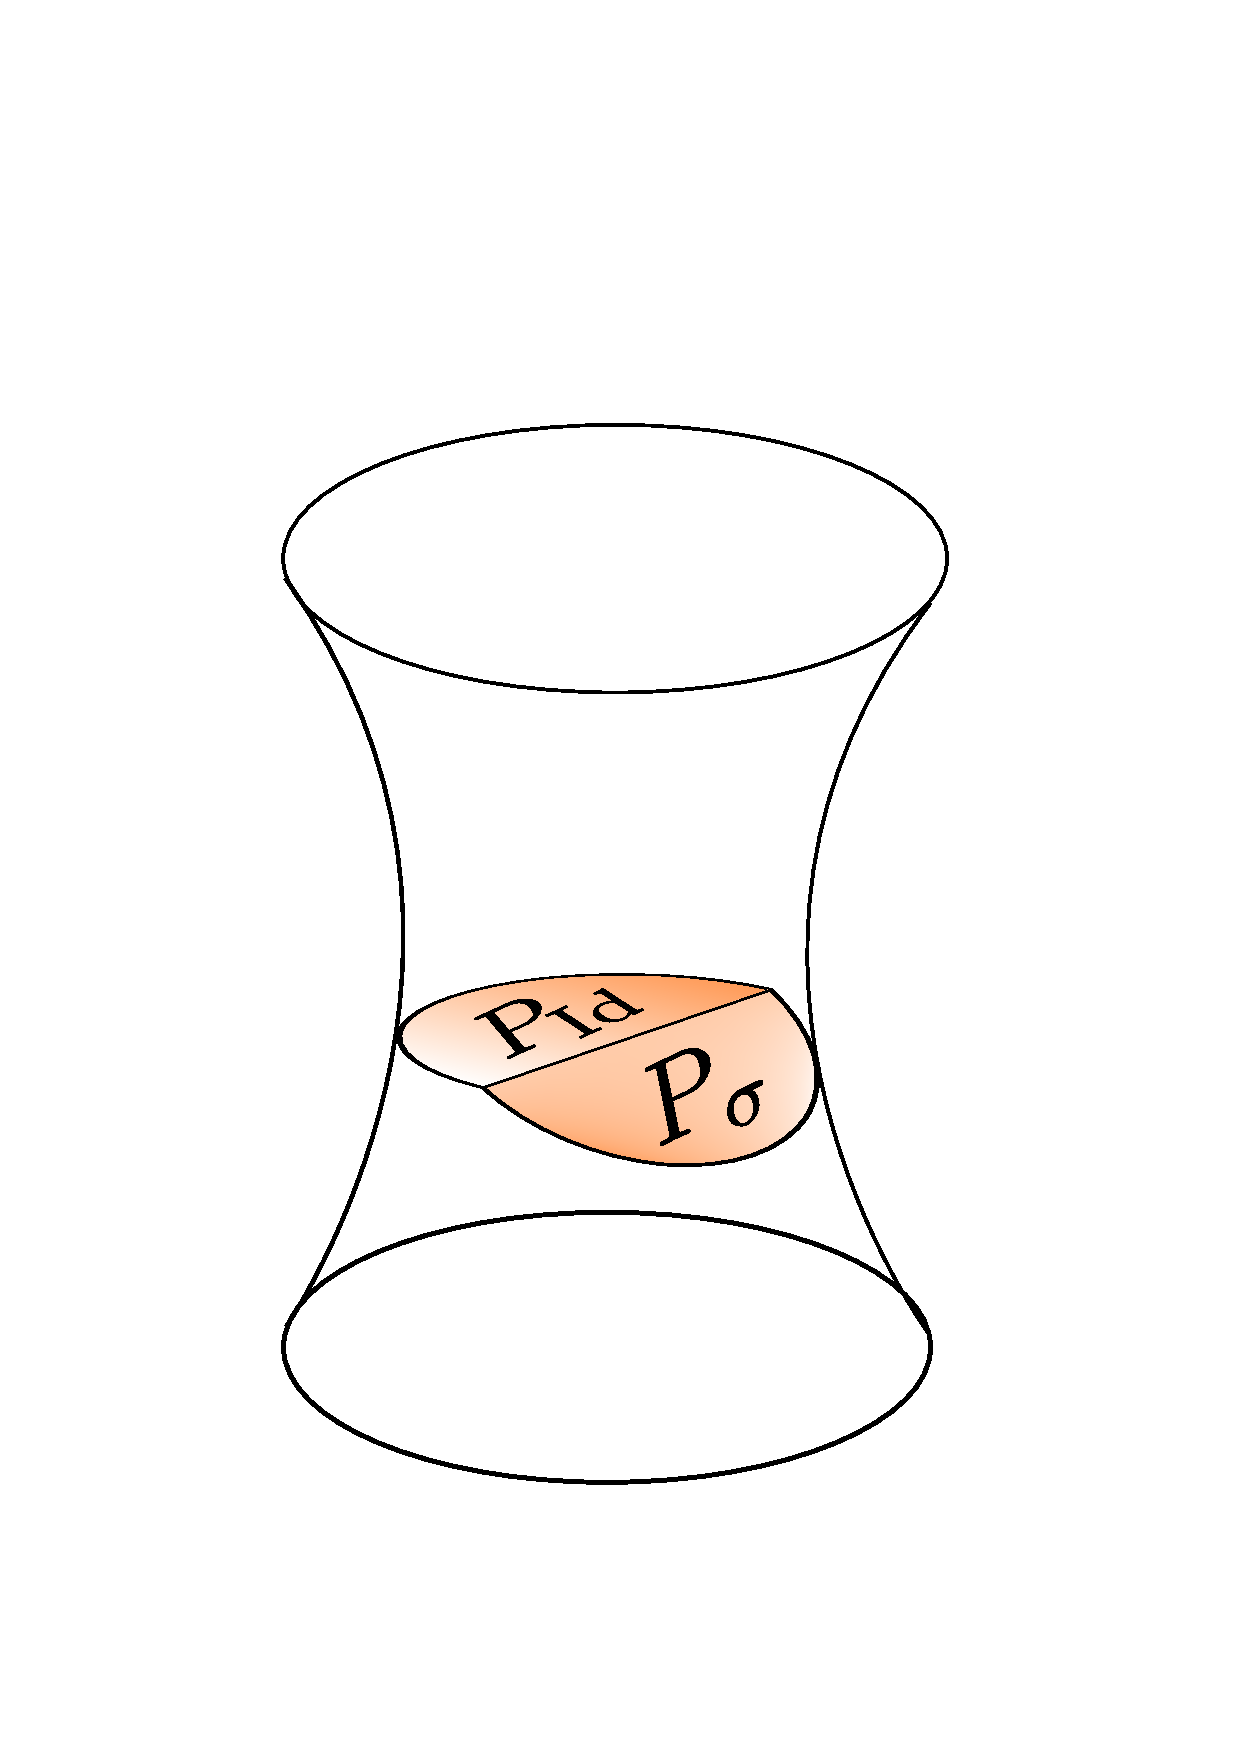
\includegraphics[width=0.5\textwidth]{bendinglocus.pdf}
    \caption{A bending surface in $\A^{2,1}$, consisting of two half-planes meeting along a common geodesic. The bending geodesic is the axis of the loxodromic isometry $\sigma$.}
    \label{pleatedinho}
\end{figure}

More in detail, the key observation that we will use is due to Mess' work \cite{Mess}, that highlighted the relation between pleated surfaces and earthquake maps. Recall that given an achronal meridian $\Lambda\subset\A^{2,1},$ the upper and lower boundary components $\partial_{\pm}\CF$ of the convex hull of $\Lambda$ are a convex and a concave pleated surface, see Proposition \ref{466}.\\
We give a brief sketch of the idea of the proof and then will fill in the details. Consider left and right projections from $\partial_+\CF$ to $\H^2,$ now the composition $\Pi_r\circ\Pi_l^{-1}$  is a left earthquake map defined in the complement of the simplicial leaves of the lamination, and its earthquake lamination is identified to the bending lamination of $\partial_{+}\CF$. A completely analogous statement holds for $\partial_{-}\CF$ by reversing the roles of left and right.\\  
Now, when the curve $\Lambda$ is the graph of an orientation-preserving homeomorphism of $\S$, one obtains as a result earthquakes maps of $\H^2$. When moreover $\varphi$ is the homeomorphism which conjugates left and right representations $\rho_l,\rho_r:\pi_1(\Sigma)\to\PSL$ of the holonomy of a MGH Cauchy compact manifold, the naturality of the construction implies that the earthquake map descends to an earthquake map from the left to the right hyperbolic surfaces, namely $\H^2/\rho_l(\pi_1(\Sigma))$ and $\H^2/\rho_r(\pi_1(\Sigma))$, and we can recover the earthquake theorem as in Kerchoff's (weaker) original formulation \cite{kerckhoff1983nielsen}.\\
Given the previous discussion, we can now start with the details.


% \section{Affine space and Convexity Notions}
% The initial step in our proof is to consider the graph of an orientation-preserving homeomorphism $f:\R\text{P}^1\to\R\text{P}^1$ as a subset of $\partial\A^{2,1}$, and taking its convex hull. However, the convex hull of a set in projective space can be defined in affine chart, but $\overline{\A^{2,1}}$ is not contained in any affine chart. The following lemma has the purpose to show that the convex hull of the graph of $f$ is well-defined: 
% \begin{lemma}\label{bdconvex}
%     Let $f:\R\text{P}^1\to\R\text{P}^1$ be an orientation-preserving homeomorphism. Then: 
%     \begin{enumerate}
%         \item There exists a spacelike plane $\text{P}_\gamma$ in $\A^{2,1}$ such that $\partial\A^{2,1}\cap\text{graph}(f)=\emptyset.$
%         \item Given any point $(x_0,y_0)\notin\text{graph}(f)$, there exists a spacelike plane $\text{P}_\gamma$ such that $\partial\text{P}_\gamma=\emptyset$ and $(x_0,y_0)\in\partial\text{P}_\gamma.$ 
%     \end{enumerate}
% \end{lemma}

% \begin{proof}
%     \begin{enumerate}
%         \item We recall that $\PSL$ acts transitively on pairs of distinct points of $\R\text{P}^1\simeq\R\cup\{\infty\}$ (actually more is true, as it acts simply transitively on \textit{positively oriented triples}). Hence we may assume, up to the action of the isometry group of $\A^{2,1}$ by post-composition on $f$ (we observe that because of equivariance given $(\alpha,\beta)\in\T$ it holds $(\alpha,\beta)\cdot\text{graph}(f)=\text{graph}(\beta f\alpha^{-1})$), that $f(0)=0$ and $f(\infty)=\infty.$ The $f$ induces a monotone increasing homeomorphism from $R\to\R$. Since $f(0)=0,$ the map $f$ preserves the two intervals: $(-\infty,0)$ and $(0,\infty).$ Let now $\gamma=\mathcal{R}_i$ be the order-two elliptic isometry fixing $i$. Clearly $\gamma$ is an involution that maps $0\to\infty,$ \todo{show this}, and switches the two intervals $(-\infty,0)$ and $(0,\infty)$. Hence $f(x)\neq\gamma(x)$ for all $x\in\R\cup\{\infty\}$, that is $\text{graph}(f)\cap\text{graph}(\gamma)=\emptyset.$ Now by lemma \textcolor{red}{cite} and the fact that $\gamma$ is an involution, $\text{graph}(f)\cap\partial\text{P}_\gamma=\emptyset.$
%         \item In proving this point we will use the aforementioned $\PSL$-transitivy on triples, and we will apply both pre and post-composition of an element of $\PSL$. We observe that if $(x_0,y_0)\notin\text{graph}(f)$, then we can find points $x,x^{\prime}$ such that $f$ maps the unoriented arc of $\R\text{P}^1$ connecting $x,x^{\prime}$ containing $x_0$ to the unoriented arc connecting $f(x),f(x^{\prime})$ \textit{not} containing $f(y_0),$ the proof is just figure \textcolor{red}{inserire la figura}. Now, since $f$ preserve the orientation of $\R\text{P}^1,$ up to switching $x,x^{\prime}$, we have that $(x, x_0, x^{\prime})$ is a positive triple in $\S$, while $(f(x),y_0,f(x^{\prime}))$ is a negative triple. \\
%         Following the observation, and using simply transitivity on oriented triples, we can assume $(x,x_0,x^{\prime})=(0,1,\infty)$ and $(f(x),y_0,f(x^{\prime}))=(0,-1,\infty).$ At this point choosing $\gamma=\mathcal{R}_i$ as in the first point of the proof satisfies the condition in the second item as well, since $\gamma(1)=-1$.  
%     \end{enumerate}
% \end{proof}

% Now, given a spacelike plane $\text{P}_\gamma$ in $\A^{2,1}$, let $\mathcal{P}_\gamma$ be the unique projective subspaces in $\text{P}\mathcal{M}(2,\R)$ that contains $\text{P}_\gamma$, which is identified by the equation \refeq{spacelike} (where now $[A]=\gamma$). Let us denote by $\mathcal{A}_\gamma$ the complement of $\mathcal{P}_\gamma$, which we will call a (\textit{spacelike}) \textit{affine chart}. In this setting the first item of the lemma \ref{bdconvex} can be riformulated as: 
% \begin{corollary}\label{affinechart}
%     Let $f:\S\to\S$ be an oriented-preserving homeomorphism. There exists a spacelike affine chart $\mathcal{A}_\gamma$ containing $\text{graph}(f)$.
% \end{corollary} 

% Resolved any matter with the good definition of convex hull of $\text{graph}(f)$ we want to understand the matter with an example: \\


% To continue in our exploration of convexity in $\A^{2,1}$ we will need one last technical Lemma similar in spirit to \ref{bdconvex}: 
% \begin{lemma}\label{convI}
%     Let $f:\S\to\S$ be and orientation-preserving homeomorphism and let $\text{P}_\gamma$ in $\A^{2,1}$ be a spacelike plane such that $\partial\text{P}_\gamma\cap\text{graph}(f)=\emptyset.$ Given any two distinct points $(x,f(x)), (x^{\prime} ,f(x^{\prime} ))$ in $\text{graph}(f)$, there exists a spacelike plane, disjoint from P$_\gamma$, containing them in its boundary at infinity. 
% \end{lemma}
% \begin{proof}
%     Acting via $\PSL\times\PSL$ we can assume that $\gamma=\text{Id}$. The hypothesis $\partial\text{P}_{\text{Id}}\cap\text{graph(f)}=\emptyset$ can be rephrased as saying that $f$ has no fixed point. We are looking for a $\sigma\in\PSL$ such that:
%     \begin{itemize}
%         \item P$_{\text{Id}}\cap\text{P}_\sigma=\emptyset$ 
%         \item $(x,f(x)),(x^{\prime} ,f(x^{\prime}))\in\partial\text{P}_{\sigma^{-1}}=\text{graph}(\sigma).$
%     \end{itemize}
%     For the first condition to hold it is suffices that the boundary of $\text{P}_{\text{Id}},\text{P}_{\sigma^{-1}}$ do not intersect, that is to say, $\sigma(y)\neq y$ for every $y\in\S$. We are then asking for a $\sigma$ with no fixed points on $\S$, namely $\sigma$ has to be an elliptic isometry. The second condition can be restated as $\sigma(x)=f(x)$ and $\sigma(x^{\prime})=f(x^{\prime}).$\\
% Now, since $f$ has no fixed points, $f(x)\neq x$ and $f(x^{\prime})\neq x^{\prime}$. There are various case to distinguish (refer to figure \textcolor{red}{inserire} for a visual aid). First we suppose for $(x,f(x),x^{\prime})$ to be a positive triple. Then either $(x,f(x^{\prime}),f(x),x^{\prime})$ or $(x,f(x),x^{\prime},f(x^{\prime}))$ are in cyclic order, because the remaining possibility, namely that $(x,f(x),f(x^{\prime}) ,x^{\prime})$ are in cyclic order, would imply that $f$ has a fix point. \todo{why so?} If $(x,f(x^{\prime}),f(x),x^{\prime})$ are in cyclic order, then the hyperbolic geodesic $\ell$ connecting $x$ to $f(x)$ and $\ell^{\prime}$ conntecting $x^{\prime} $ to $f(x^{\prime})$ must intersect, and the order two elliptic isometry $\sigma$ fixing $\ell\cap\ell^{\prime}$ maps $x\to f(x)$ and $x^{\prime} \to f(x^{\prime})$.\\
% If $(x,f(x),x^{\prime},f(x^{\prime}))$ are in cyclic order, then the geodesic $\ell_1$ connecting $x$ to $x^{\prime}$ and the geodesic $\ell_2$ connecting $f(x)$ to $f(x^{\prime})$ must intersect and one can find an elliptic element $\sigma$ fixing $\ell_1\cap\ell_2$ sending $x\to f(x)$ and $x^{\prime} \to f(x^{\prime}).$ Second, if $(x,f(x),x^{\prime} )$ is a negative triple, then the argument works \textit{verbatim}. Finally, there is the possibility that $f(x)=x^{\prime}$. If $f(x^{\prime})\neq f(x)$, the $\sigma$ we are looking for is an order-three elliptic isometry with fixed point in the barycenter of the triangle of vertices $x,f(x)=x^{\prime},f(x^{\prime})$. If $f(x^{\prime})=x$, we run out of cases by taking as $\sigma$ the order-two elliptic isometry with fixed point on the geodesic $\ell$ from $x$ to $x^{\prime}$. \\
% \end{proof}

% In particular, as a consequence of Lemma \ref{convI}, we have that given any spacelike affine chart $\mathcal{A}_\gamma$ containing $\text{graph}(f)$ and any two distinct points in $\text{graph}(f)$ the line connecting them is contained in $\A^{2,1}\cap\mathcal{A}_\gamma$ (excepts for the endpoints, which are in $\partial\A^{2,1}$), and it is a spacelike geodesic of $\A^{2,1}$.\\
% We are now ready to prove the following: 
% \begin{proposition}\label{convII}
%     Let $f:\S\to\S$ be an orientation-preserving homeomorphism, let $\text{P}_\gamma$ in $\A^{2,1}$ be a spacelike plane such that $\partial\text{P}_\gamma\cap\text{graph}(f)=\emptyset,$ and let $K$ be the convex hull of $\text{graph}(f)$ in the affine chart $\mathcal{A}_\gamma$. Then: 
%     \begin{itemize}
%         \item The interior of $K$ is contained in $\A^{2,1}$
%         \item The intersection of $K$ with $\partial\A^{2,1}$ is equal to $\text{graph}(f)$.
%     \end{itemize}
%     In particular, $K$ is a convex body that is a subset of $\overline{\A^{2,1}}$.
% \end{proposition}
% \begin{proof}
%     Given a point in $\partial\A^{2,1}\setminus\text{graph}(f)$, by the second item of Lemma \ref{bdconvex} there exists a spacelike plane $\text{P}_\eta$ passing through $p$ that does not intersect $\text{graph}(f).$ This implies $\text{P}_\eta\cap K=\emptyset,$ hence $K\cap\partial\A^{2,1}=\text{graph}(f).$ Since $K$ is connected, it is contained in the closure of one component of the complement of $\partial\A^{2,1}$ in $\mathcal{A}_\gamma.$ But $K$ is connected and intersects $\A^{2,1}\setminus\text{P}_\gamma$ because, by \ref{convI}, the line segment connecting any two point of $\text{graph}(f)$ in the affine chart $\mathcal{A}_\gamma$ is contained in $\A^{2,1}\cap\mathcal{A}_\gamma.$ Hence $K$ is contained in $\overline{\A^{2,1}}$ with interior in $\A^{2,1}$. \\
% \end{proof}

% In light of Corollary \ref{affinechart} and Proposition \ref{convII}, we give the following definition: 
% \begin{definition}
%     Let $f:\S\to\S$ be an orientation-preserving homeomorphism, we define $\mathcal{C}(f)$ to be the subset of $\overline{\A^{2,1}}$ that is the convex hull of $\text{graph}(f)$ in any spacelike affine chart $\mathcal{A}_\gamma$ such that $\partial\text{P}_\gamma\cap\text{graph}(f)=\emptyset.$
% \end{definition}

% The definition is well-posed because lines and planes are well-defined in projective space, hence the change of coordinates from an affine chart to another preserves convex sets. Because of this when referring to convexity notion in the following, we will implicitly assume that we have chosen a spacelike affine chart $\mathcal{A}_\gamma$ that contains $\text{graph}(f)$.

\section{Earthquake Theorem}\label{quakesection}
We consider $\varphi:\S\to\S$ an orientation-preserving homeomorphism of the circle, and by $\Lambda_\varphi$ we denote its graph as a subset of $\T$ identified as $\partial\A^{2,1}$. We recall that with the notation of the previous chapter, $\Lambda_\varphi$ is a properly achronal meridian. By means of the Gauss map we had defined left and right projections for $\mathcal{C}^1$ embeddings.
% \[
%     \Pi_l^{\pm:}\partial_\pm\CF\to\H^2 \;\;\; \Pi_r^{\pm:}\partial_\pm\CF\to\H^2.
% \]
Now we would like to extend the Gauss map even when we have weaker regularity condition. Consider a point $p \in \partial_\pm\CF$ and let $P$ be a support plane of $\CF$ at $p$. By Proposition \ref{supportinho} the support plane is necessarily spacelike, hence of the form $P=P_\gamma$ for some $\gamma\in\PSL$. What happens when $\partial_\pm\CF$ is not $C^1$ at $p$ is that we do not have a unique support plane. Hence we \textit{choose} a support plane $P_\gamma$ at $p$, requiring that the choice of support planes is made so that the support plane is constant on any connected component of the subset of $\partial_\pm\CF$ consisting of those points that admit more than one support plane. The definition of the Gauss map then \textit{depends} on the choice of $P_\gamma$ (see Corollary \ref{multipleplanes} for more details on how the choice influences the map). Once we have chosen the support planes we can just follow \textit{verbatim} the construction of the Gauss map given in the smooth case.

% \section{Left and right projections.} We want to introduce two maps, \textit{left and right projections,} which will have a key role in the proof of the earthquake theorem. These are the maps: 
% \[
%     \Pi_l^\pm:\partial_\pm\CF\to\H^2 \;\;\; \Pi_r^\pm:\partial_\pm\CF\to\H^2
% \] 

% defined on the past or future of $\partial\CF$ constructed as follows. Given a point $p\in\partial_\pm\CF$, let $P$ be a support plane of $\CF$ at $p$. By Proposition \textcolor{red}{ref}, the support plane is necessarily spacelike, hence of the form $P=P_\gamma$ for some $\gamma\in\PSL$.

 %\begin{observation}
 %We have shown the existance of such a $P_\gamma$ but in general it might not be unique, if $\partial_{\pm}\CF$ is not $C^1$ at $p.$ Hence we \textit{choose} a support plane $P_\gamma$ at $p$. We also require that the choice of support plane is made so that the support plane is constant on any connected components of the subsets of $\partial_\pm\CF$ consistings of points that admit more than one support plane. The definitions of the projection then \textit{depends} (we will shortly characterize how in \textcolor{red}{add}) on the choice of $P_\gamma$.
 %\end{observation}

% Now, we choose a support plane $P_\gamma$ at $p$, left or right multiplication by $\gamma^{-1}$ maps $\gamma$ to the identity, and therefore it maps $P_\gamma$ to $P_{\text{Id}},$ which we have already studied in \textcolor{red}{reference} it is the space of order-two elliptic elements and is therefore naturally identified with $\H^2$ via the map: $\text{Fix}:P_{\text{Id}}\to\H^2.$ \\
% In classic Lie group theory fashion we denote by $L_{\gamma^{-1}}:\PSL\to\PSL$ and $\R_{\gamma^{-1}}:\PSL\to\PSL$ the left and right multiplication by $\gamma^{-1}$; these can also be viewed as the action of the elements $(\gamma,\text{Id})$ and $(\text{Id},\gamma^{-1})$ of $\PSL\times\PSL$. We now have that both $L_{\gamma^{-1}}(p)$ and $R_{\gamma^{-1}}(p)$ are elements of $P_{\text{Id}}$ and $L_{\gamma^{-1}}(p)$ (resp. $R_{\gamma^{-1}}(p)$) is a bijection between $P_\gamma$ and $P_\text{Id}.$ We can now define: 
% \begin{equation}\label{defproj}
%     \Pi_l^\pm(p)=Fix(R_{\gamma^{-1}}(p))\;\ \Pi_r^\pm(p)=Fix(L_{\gamma^{-1}}(p)).
% \end{equation}
    


% The choice of define left and right projection in this apparently counterintuitive way is motivated by the following:

% \begin{lemma}
%     Let $f:\S\to\S$ be an orientation-preserving homeomorphism, and let $(\alpha, \beta)\in \PSL\times\PSL$. Let us denote $K=\CF$ and $\hat{K}=(\alpha,\beta)\cdot\CF$ and let, $\Pi_l^{\pm},\Pi_r^{\pm}:\partial_{\pm}K\to\H^2$ and $\hat{\pi}_l^\pm,\hat{\pi}_r^\pm:\hat{K}\to\H^2$ be the left and right projection of $K$ and $\hat{K}$ respectively. Then:
%     \begin{equation}\label{equivariance}
%         \hat{\pi}_l^\pm\circ(\alpha,\beta)=\alpha\circ\Pi_l^\pm\;\;\;\ \hat{\pi}_r^\pm\circ(\alpha,\beta)=\beta\circ\Pi_r^\pm.
%     \end{equation}
% \end{lemma}
% Let's clarify the statement. The isometry $(\alpha,\beta)$ maps a point $p\in K$ to a point $\hat{p}\in\hat{K}$, and maps support planes at $p\in K$ to support planes at $\hat{p}$. Hence the relation introduced in \refeq{equivariance} holds when we consider the projections $\hat{\pi}_l^\pm$ and $\Pi_r^\pm$ defined with the choice of support planes of $\hat{K}$ given by the images $\hat{P}$ chosen in the definitions of $\Pi_l^\pm$ and $\Pi_r^\pm$.

% \begin{proof}
%     We recall that for any $\pi \in \partial^\pm K$, we consider $\hat{p}\coloneqq(\alpha,\beta)\cdot p\in\hat{K},$ and for a chosen support plane $P=P_\gamma$ for $K$ at $p,$ $(\alpha,\beta)\cdot P=P_{\hat{\gamma}}$ is the chosen support plane for $\hat{K}$ at $\hat{p}.$\\
%     By the duality, $\hat{\gamma}=(\alpha,\beta)\cdot\gamma=\alpha\gamma\beta^{-1}.$ It follows that: 
%     \begin{align*}
%         \hat{\pi}_l^\pm(\hat{p}) &= \text{Fix}(R_{\hat{\gamma}^{-1}}(\hat{p}))=\text{Fix}(R_{(\beta\gamma^{-1}\alpha^{-1})}(\alpha p\beta^{-1}))\\
%         &=\text{Fix}(R_{(\gamma^{-1}\alpha^{-1})}(\alpha p))=\text{Fix}(\alpha\circ R_{\gamma^{-1}}(p)\circ\alpha^{-1}) \\
%         &=\alpha(\text{Fix}(R_\gamma^{-1})(p))=\alpha\circ\Pi_l^\pm(p).
%     \end{align*}
%     And a completely analogous argument holds for the right projection.
% \end{proof}

\begin{example}\label{413} Let us consider a toy case where $\varphi\in\PSL$ so that $\CF=P_{\varphi^{-1}}$ as in the previous Example \ref{43}. This is in some sense a degenerate case, as $\CF$ has empty interior, hence Corollary \ref{nametag} does not apply and it does not \textit{really} make sense to talk about the future and the past component boundary. However, we can still define a left and right projections. Since $P_{\varphi^{-1}}$ itself is the unique support plane at any of its points, from the definition of the Gauss map we have the following expressions for the left and right projection $\Pi_l,\Pi_r:P_{\varphi^{-1}}\to\H^2:$
\begin{equation}\label{12}
    \Pi_l(p)=\text{Fix}(p\circ\varphi)\;\;\Pi_r(p)=\text{Fix}(\varphi\circ p).
\end{equation}   
We can also extend the two maps to the boundary of $P_{\varphi^{-1}}$: recalling that its boundary coincides with the graph of $\varphi$ (Lemma \ref{32}) we have: 
\begin{equation}\label{simproj}
    \Pi_l(x,\varphi(x))=x \;\;\;\Pi_r(x,\varphi(x))=\varphi(x). 
\end{equation}

Equation \refeq{simproj} is immediately checked when $\varphi=\text{Id},$ because in that case we have that $\Pi_l,\Pi_r$ simply coincide with the fixed point map $\text{Fix}:P_{\text{Id}}\to\H^2$, and we observed previously that $\text{Fix}$ extends to the map $(x,x)\to x$ from $\partial P_{\text{Id}}$ to $\partial\H^2$. The general case of Equation \refeq{simproj} is then consequence of the equivariance of the Gauss map, with the additional observation that the isometry $(\text{Id},\varphi)$ maps $\text{graph}(\text{Id})$ to $\text{graph}(\varphi)$ and $P_\text{Id}$ to $P_{\varphi^{-1}}$. \\
We can now compute the map of $\H^2$ obtained by composing the inverse of the left projection with the right projection. Indeed, this is induced by the map $P_{\text{Id}}\to P_\text{Id}$ sending an order-two elliptic element $\mathcal{R}=p\circ\varphi\in P_{\text{Id}}$ to $\varphi\circ p=\varphi\circ\mathcal{R}\circ\varphi^{-1}$. Hence we have   
\begin{equation}\label{composition}
    \Pi_r\circ\Pi_l^{-1}=\varphi:\H^2\to\H^2.
\end{equation}
In conclusion, we have that the composition of the maps $\Pi_r\circ\Pi_l^{-1}$ is an isometry and its extension to the boundary of $\H^2$ is precisely the map $f=\varphi$ of which $\partial P_{\varphi^{-1}}$ is the graph. In what follows we will observe that this is what happens in the general case, that is, given an orientation-preserving homeomorphism of the circle $\varphi$, the composition $\Pi_r^\pm\circ(\Pi_l^\pm)^{-1}$ associated with $\partial_\pm\CF$ will be the left and right earthquake extending $\varphi$.
\end{example}

\section{The fundamental example}\label{fundamentalexamplesec} We want to move one more intermediate step towards the final theorem. After the simple case, this time we will describe what we can consider \textit{the fundamental example}. Consider piecewise totally geodesic surfaces in $\A^{2,1},$ which are obtained as the union of two connected subsets, each contained in a totally geodesic spacelike plane, meeting along a common geodesic. \\
Let us formalize this idea in a more precise way. Consider the union of two half-planes, each contained in a totally geodesic spacelike plane $P_{\gamma_1},P_{\gamma_2}$. The first key fact is the following:

\begin{lemma}\label{Mati}
    Let $\gamma_1\neq\gamma_2\in\PSL$. Then $P_{\gamma_1}$ and $P_{\gamma_2}$ intersect in $\A^{2,1}$ if and only if $\gamma_2\circ{\gamma_1^{-1}}$ is a loxodromic isometry. 
\end{lemma}
\begin{proof}
    As in Example \ref{43}, $P_{\gamma_i}$ is the convex hull of $\partial P_{\gamma_i}=\text{graph}(\gamma_i^{-1}),$ the closures $\overline{P}_{\gamma_i}$  intersect in $\overline{\A^{2,1}}$ if and only if $\text{graph}(\gamma_1)\cap\text{graph}(\gamma_2)\neq\emptyset$. Moreover, by Equation \refeq{suplane}, $P_{\gamma_1}$ and $P_{\gamma_2}$ intersect in $\A^{2,1}$ if and only if $\text{graph}(\gamma_1)\cap\text{graph}(\gamma_2)$ contains at least two different points. \\
    We know that $(x,y)\in\T$ is in $\text{graph}(\gamma_1)\cap\text{graph}(\gamma_2)$ if and only if $y=\gamma_1^{-1}(x)=\gamma_2^{-1}(x)$, which is equivalent to asking that $x\in\text{Fix}(\gamma_2\circ\gamma_1^{-1})$. But the composition $\gamma_2\circ\gamma_1^{-1}$ is an element of $\PSL$, hence it has two fixed points in $\partial\H^2\simeq\S$ if and only if it is a loxodromic isometry.
\end{proof}


Now consider $\S=I_1\cup I_2$ where $I_1,I_2$ are two closed intervals such that $I_1\cap I_2$ consists exactly of the two fixed points of $\gamma_2\circ\gamma_1^{-1}.$ There are two possibilities to produce a homeomorphism of $\S$ by composing the restriction of $\gamma_1^{-1}$ and $\gamma_2^{-1}$ to the intervals $I_j$'s, namely: 

\begin{equation}\label{17}
    \varphi_{\gamma_1,\gamma_2}^+(x) = \begin{dcases}
        \gamma_1^{-1}, & \text{if } x \in I_1 \\
        \gamma_2^{-1}, & \text{if } x \in I_2
    \end{dcases}
    \;\text{and}\;
    \varphi^-_{\gamma_1,\gamma_2}(x) = \begin{dcases}
        \gamma_2^{-1}, & \text{if } x \in I_1 \\
        \gamma_1^{-1} , & \text{if } x \in I_2
    \end{dcases}.
    \end{equation}
    
    Both $\varphi_{\gamma_1,\gamma_2}^{\pm}$ are orientation-preserving homeomorphism, since $\gamma_1^{-1}$ and $\gamma_2^{-1}$ map homeomorphically the intervals $I_1$ and $I_2$ to the same intervals $J_1\coloneqq\gamma_1^{-1}(I_1)=\gamma_2^{-1}(I_1)$ and $J_2\coloneqq\gamma_1^{-1}(I_2)=\gamma_2^{-1}(I_2)$ which intersects only at their endpoints. \\
    We denote by $D_i$ the convex hull of $I_i$ in $\H^2,$ and by $\ell=D_1\cap D_2$ the axis of $\gamma_2\circ\gamma_1^{-1}$. 
    % We observe that the projections $\Pi_l, \Pi_r$ are well defined isometries on each (totally geodesic) connected component of the complement of such bending geodesic in $S$. We may assume that $D_1$ is contained in the plane $P_{\text{Id}}$, which we recall consisting of order two-elliptic elements of $\PSL$. Therefore the bending locus is a spacelike geodesic contained in $P_{\text{Id}}$, namely the set of order-two elliptic elements of $\PSL$ having fixed point in a geodesic $\ell$ of $\H^2$. \\ 
    % With the notation that we introduced in Section \ref{geosection}, it has the form: 
    % \[
    %     L_{\ell,\ell^{\prime}}=\{X\in\PSL\;|\;X\cdot\ell^{\prime} =\ell\; \text{as oriented geodesic}\}, 
    % \]
    % where $\ell^{\prime}$ is the geodesic having the same support of $\ell$ but the opposite orientation. The stabilizer of this spacelike geodesic is a subgroup of $\PSL\times\PSL$ isomorphic to $\R^2$ and consisting of pairs $(A,B)\in\PSL\times\PSL$ where both $A,B$ are loxodromic isometries preserving $\ell$. The stabilizer of $L_{\ell,\ell^{\prime}}$ fixes (setwise) also the dual geodesic $L_{\ell,\ell}$ as in Remark \ref{355}. \\
    % Actually more is true, it follows from the definition of dual geodesic that the dual point of the spacelike plane $D_2$ lies in the dual geodesic, and it is therefore a loxodromic transformation $\sigma_0$ with axis $\ell$. Now, it follows from the definition of the Gauss map that the left projection: \(\Pi_l:D_1\cup D_2\to\H^2\) is the identity on $D_1$ (we remark that we identify $P_{Id}$ with an isometric copy of $\H^2$), while on $D_2$ it is given by the multiplication on the right by $\sigma_0^{-1}$. Similarly, the right projection is the identity on $D_2$ and the multiplication on the left by $\sigma_0^{-1}$ on $D_2$.\\
    % In conclusion, the composition $\Pi_r\circ\Pi_l^{-1}$ acts on $P_{\text{Id}}$ as the identity on one connected component of the complement of $L_{\ell,\ell^{\prime}}$ and conjugates by $\sigma_0$ on the other connected components, which simply means acting by the loxodormic transformation $\sigma_0$ under the identification of $P_{\text{Id}}$ with $\H^2$.\\
    % This is exactly the simple earthquake map with associated geodesic lamination $\ell$. Since the angle between the spacelike planes containing $D_1$ and $D_2$ equals the distance in the dual geodesic $L_{\ell,\ell}$ between the corresponding dual points, we also conclude that the bending measure equals the measure associated with the earthquake map (this will not be used as we are interested only in closed surfaces but shows how we could recover the \textit{full} Thurston's theorem from AdS geometry as in \cite{benedetti2009canonical}). The bending and earthquake lamination are identified. 

    
 \begin{proposition}\label{gettinthere}
    Suppose that $\gamma_2\circ\gamma_1^{-1}$ is a loxodromic isometry that translates along $\ell$ to the left, as seen from $D_1$ to $D_2$. Then:
     \begin{itemize}
         \item The future boundary component $\partial_+\mathcal{C}(\varphi_{\gamma^+,\gamma_2}^{+})$ coincides with the union of the convex envelope of $\text{graph}(\restr{\gamma_1^{-1}}{I_1})$ and the convex envelope of $\text{graph}(\restr{\gamma_2^{-1}}{I_2}).$
         \item The past boundary component $\partial_-\mathcal{C}(\varphi^-_{\gamma_1,\gamma_2})$ coincides with the union of the convex envelope of $\text{graph}(\restr{\gamma_1^{-1}}{I_2})$ and of the convex envelope of $\text{graph}(\restr{\gamma_2^{-1}}{I_1}).$
    \end{itemize}
    If instead $\gamma_2\circ\gamma_1^{-1}$ translates along $\ell$ to the right as seen from $D_1$ to $D_2$, then:
    \begin{itemize}
         \item The past boundary component of $\partial_-\mathcal{C}(\varphi_{\gamma_1,\gamma_2}^+)$ coincides with the union of the convex envelope of $\text{graph}(\restr{\gamma_1^{-1}}{I_1})$ and of the convex envelope of $\text{graph}(\restr{\gamma_2^{-1}}{I_2})$. 
         \item The future boundary component $\partial_+\mathcal{C}(\varphi_{\gamma_1,\gamma_2}^-)$ is the union of the convex envelope of $\text{graph}(\restr{\gamma_1^{-1}}{I_2})$ and of the convex envelope of $\text{graph}(\restr{\gamma_2^{-1}}{I_1}).$
     \end{itemize}
 \end{proposition}

 \begin{proof}
     Let us consider the case where $\gamma_2\circ\gamma_1^{-1}$ translates to the left along $\ell$, and let us prove the first item. Let $x,x^{\prime}$ be the fixed points of $\gamma_2\circ\gamma_1^{-1},$ let $y=\gamma_1^{-1}(x)=\gamma_2^{-1}(x)$ and $y^{\prime}=\gamma_1^{-1}(x^{\prime})=\gamma_2^{-1}(x^{\prime})$. Then the convex envelope of graph($\restr{\gamma_i^{-1}}{I_i}$) is a half-plane $A_i$ in $P_{\gamma_i}$ bounded by the geodesic $P_{\gamma_1}\cap P_{\gamma_2}$, which has endpoints $(x,y)$ and $(x^{\prime} ,y^{\prime})$, Clearly both the convex envelope of graph($\restr{\gamma_i^{-1}}{I_i}$) are contained in $\mathcal{C}(\varphi_{\gamma_1,\gamma_2}^{+}).$\\
     We could be even more precise. We claim that $P_{\gamma_1}$ and $P_{\gamma_2}$ are future support planes for $\mathcal{C}(\varphi_{\gamma_1,\gamma_2}^{+})$. The claim will imply that the union of $A_1$ and $A_2$ is contained in the future boundary component $\partial_+\mathcal{C}(\varphi_{\gamma_1,\gamma_2}^{+})$, because every point $p\in A_1\cup A_2$ admits a future support plane through $p$ which is either $P_{\gamma_1}$ or $P_{\gamma_2}$. However $A_1\cup A_2$ is a topological disc in $\partial_+\mathcal{C}(\varphi_{\gamma_1,\gamma_2}^{+}),$ whose boundary is precisely the curve $\text{graph}(\varphi_{\gamma_1,\gamma_2}^{+})$ by construction. Hence the claim will imply that $A_1\cup A_2=\partial_+(\varphi_{\gamma_1,\gamma_2}^{+}).$\\
     We prove the claim for $P_{\gamma_1}$, proof for $P_{\gamma_2}$ is analogous. For convenience we set $\gamma_1=\text{Id}$ and $\gamma_2=\gamma$ is a loxodromic isometry with fixed points $x,x^{\prime}$, translating to the left as seen from $D_1$ to $D_2$. Indeed, we can reach such a configuration by applying $(\text{Id},\gamma_1),$ which sends $P_{\gamma_1}$ to $P_1$, $P_{\gamma_2}$ to $P_{\gamma_2\gamma_1^{-1}}$, and graph($\varphi_{\gamma_1,\gamma_2}^+$) to graph($\varphi_{\text{Id},\gamma_2\gamma_1^{-1}}^+$). \\
     We can now consider a path $\sigma_t,$ for $t\in[0,\epsilon]$ of elliptic elements fixing a given point $z_0\in\H^2,$ that rotate clockwise by an angle $t.$ As in the proof of Lemma \ref{Mati} the planes $P_{\sigma_t}$ are pairwise disjoint in $\overline{\A^{2,1}}$, because $\sigma_{t_2}\circ\sigma_{t_1}^{-1}$ is still an elliptic element fixing $z_0$ for $t_1\neq t_2$, hence it has no fixed points in $\S$. Moreover recall that $\gamma^{-1}$ has a fixed axis $\ell$ and translates along $\ell$ to the right as seen from $D_1$ to $D_2$. Now $\varphi_{\text{Id},\gamma}^+$ equals the identity on $I_1$ and $\gamma_2$ on $I_2,$ it fixes $I_1$ pointwise and moves points on $I_2$ clockwise. It follows that the equation $\varphi_{\text{Id},\gamma}^+(x)=\gamma_t^{-1}(x)$ has no solution for $t>0$, because $\sigma_{t}^{-1}=\sigma_{-t}$ moves all the points counterclockwise if $t$ is positive. This shows that $P_{\sigma_t}\cap\mathcal{C}(\varphi^+_{\text{Id},\gamma})=\emptyset$ for $t>0,$ and thus $P_{\text{Id}}$ is a support plane for $\mathcal{C}(\varphi^+_{\text{Id},\gamma})$ by Remark \ref{diffsupp}.\\
     Moreover if it is a future support plane: indeed one can check that $\sigma_{t+\pi/2}=\mathcal{R}_{z_0}\circ\sigma_t\in P_{\sigma_t}$, and the path $t\mapsto\sigma_t$ is future-directed because, from the discussion after \refeq{tangent}, its tangent vector is future-directed, hence $\mathcal{C}(\varphi_{\text{Id},\gamma}^+)$ is locally in the past of $P_{\text{Id}}$. \\
     We have shown the first item of the proposition, all the others follow with completely analogous arguments.
 \end{proof}



We want to put more focus on some elements of the proof that will be exploited in the following:
 \begin{corollary}\label{53}
    Suppose that $\gamma_2\circ\gamma_1^{-1}$ is a loxodromic isometry that translates along $\ell$ to the left (resp. right), as seen from $D_1$ to $D_2$, and write $\gamma_2\circ\gamma_1^{-1}=\exp(\mathfrak{a})$ for some $\mathfrak{a}\in\mathfrak{sl}(2,\R)$. Let $p$ be a point in the future (resp. past) boundary components of $\mathcal{C}(\varphi_{\gamma_1,\gamma_2}^{+}).$ Then:
    \begin{itemize}
        \item If $p\in\text{int}(A_1)$, then $P_{\gamma_1}$ is the unique support plane of $\mathcal{C}(\varphi_{\gamma_1,\gamma_2}^{+})$ at $p$. 
       \item If $p\in\text{int}(A_2)$, then $P_{\gamma_2}$ is the unique support plane of $\mathcal{C}(\varphi_{\gamma_1,\gamma_2}^{+})$ at $p$. 
       \item If $p\in A_1\cap A_2= P_{\gamma_1}\cap P_{\gamma_2}$, then the support planes of $\mathcal{C}(\varphi_{\gamma_1,\gamma_2}^{+})$ at $p$ are precisely those of the form $P_{\sigma\gamma_1}$ where $\sigma=\text{exp}(t\mathfrak{a})$ for $t\in [0,1].$  
   \end{itemize}

    
 \end{corollary}

 We are still using the notation introduced in the fundamental example: $A_i\subset P_{\gamma_i}$ is the convex envelope of $\text{graph}(\restr{\gamma_i^{-1}}{I_i}$), an half-plane bounded by the geodesic $P_{\gamma_1}\cap P_{\gamma_2}.$ As expected a completely analogous statement could be formulated for $\mathcal{C}(\varphi_{\gamma_1,\gamma_2}^{-})$ but we restrict to the study of $\varphi_{\gamma_1,\gamma_2}^{+}$ for simplicity. 

 \begin{proof}
     The pleated surface that we obtained as the union of $A_1\subset P_{\gamma_1}$ and $A_2\subset P_{\gamma_2}$ coincides with $\partial_+\mathcal{C}(\varphi_{\gamma_1,\gamma_2}^+)$ if $\gamma_2\circ\gamma_1^{-1}$ is a loxodromic isometry that translates along $\ell$ to the left, and with $\partial_-\mathcal{C}(\varphi_{\gamma_1,\gamma_2}^+)$ if it translates to the right, as we saw in the previous example. \\
    The first two items are then clear, since $P_{\gamma_i}$ are smooth surfaces, hence $A_i$ is smooth at any interior point, and therefore has a unique support plane at the point. For the last item we can assume $\gamma_1=\text{Id}$ and $\gamma_2=\gamma$ is a loxodromic isometry translating on the left (resp. right) along $\ell.$ By Equation \refeq{suplane}, if $P_\sigma$ is a support plane at $p,$ then $p$ is in the convex hull of the pairs $(y,\sigma^{-1}(y))$ where $y$ satisfies the relation $\sigma^{-1}(y)=\varphi_{\text{Id},\gamma}^{\pm}(y).$ The only possibility is then for $p$ to lie in the geodesic connecting the points $(x,x)$ and $(x^{\prime},x^{\prime})$ in $\T,$ where $x,x^{\prime}$ are the fixed points of $\gamma$. Hence $\sigma$ must have the same fixed point as $\gamma$. It follows that $\sigma$ is then a loxodromic isometry with axis $\ell$ (or the identity). Moreover, $P_\sigma$ is in the future (resp. past) of $\mathcal{C}(\varphi_{\gamma_1,\gamma_2}^+)$ if and only if $\sigma$ translates on the left (resp. right), and its translation length is less than that of $\gamma.$ Hence $\gamma$ is of the form $\exp(t\mathfrak{a})$ for $t\in [0,1].$
\end{proof}


 We are finally arrived to the case of considering orientation-preserving homeomorphism obtained by combining two elements of $\PSL$. We want to show that in a similar setting the composition of the projections $\Pi_l^{\pm}$ and $\Pi_r^\pm$ provide the earthquake map as in Example \ref{simplequake}. At first glance this does not seem like a huge achievement as we are just recovering a simple earthquake map that we were already able to define explicitly. Nevertheless, the following proposition will be a key step to complete the proof of the earthquake theorem. 

 \begin{proposition}\label{estensione}
     Let $\gamma_1,\gamma_2 \in \PSL$ be such that $\gamma_2\circ\gamma_1^{-1}$ is a loxodromic isometry, and let $\Pi_l^\pm, \Pi_r^\pm$ be the projections associated with the convex envelope of $\varphi_{\gamma_1,\gamma_2}^+.$ Then:
     \begin{enumerate}
         \item $\Pi_l^\pm, \Pi_r^\pm:\partial_\pm\mathcal{C}(\varphi_{\gamma_1,\gamma_2}^+)\to\H^2$ are bijections.
         \item Assume that $\gamma_2\circ\gamma_1^{-1}$ translates along $\ell$ to the right (resp. left), as seen from $D_1$ to $D_2.$ Then the composition $\Pi_r^-\circ(\Pi_l^-)^{-1}:\H^2\to\H^2$ (resp. $\Pi_r^+\circ(\Pi_l^+)^{-1}:\H^2\to\H^2)$ is a left (resp. right) earthquake map extending $\varphi_{\gamma_1,\gamma_2}^+.$
     \end{enumerate} 
 \end{proposition}

 We remark that we are limiting to the case of $\varphi_{\gamma_1,\gamma_2}^+$ for simplicity and completely analogous results could be formulated in terms of $\varphi_{\gamma_1,\gamma_2}^-.$ Before proving it we remark that proposition \ref{estensione} holds for \textit{any choice}  of support planes that is needed to define the projections.

 \begin{proof}
     For the first point, recall that $A_i\subset P_{\gamma_i}$, and that the union $A_1\cup A_2$ is the past (resp. future) boundary component for $\varphi_{\gamma_1,\gamma_2}^+$ if $\gamma_2\circ\gamma_1^{-1}$ translates along $\ell$ to the right (resp. left). \\
     Hence $\restr{(\Pi_l^\pm)}{\text{int}(A_i)}$ and $\restr{(\Pi_r^\pm)}{\text{int}(A_i)}$ are the restrictions of the projections associated with the totally geodesic plane $P_{\gamma_i}$ just as seen in Example \ref{413}. In particular, $\restr{(\Pi_l^\pm)}{\text{int}(A_i)}$ and $\restr{(\Pi_r^\pm)}{\text{int}(A_i)}$ are the restriction to int($A_i$) of global isometries of $\A^{2,1}$ (those defined by multiplication on the left or on the right by $\gamma_i^{-1}$) sending $P_{\gamma_i}$ to $P_{\text{Id}}$, post-composed with the usual isometry $\text{Fix}:P_{\text{Id}}\to\H^2$. It follows that the restrictions of projections map geodesic of $P_{\gamma_i}$ to geodesic of $\H^2$. More is true, due to Equation \refeq{simproj}, $\restr{(\Pi_l^\pm)}{\text{int}(A_i)}$ maps int($\partial(A_i))=\text{graph(\restr{\gamma_i^{-1}}{\text{int}(I_i)})}$ to $\text{int}(I_i).$ Hence $\Pi_l^\pm(\text{int}(A_i))=\text{int}(D_i)$. In similar fashion, $\Pi_r^\pm(\text{int}(A_i))=\gamma_1^{-1}(\text{int}(D_1))=\gamma_2^{-1}(\text{int}(D_2)).$\\
  We want to show that the projections are bijective. To do so we will show that the image of the geodesic $A_1\cap A_2=P_{\gamma_1}\cap P_{\gamma_2}$, via $\Pi_l^\pm$ is the geodesic $\ell=D_{1}\cap D_2$, while the image via $\Pi_r^\pm$ is the geodesic $\gamma_1^{-1}(\ell)=\gamma_2^{-1}(\ell).$ The definition of $\Pi_l^\pm$ and $\Pi_r^\pm$ on $A_1\cap A_2$ \textit{depends} on the choice of a support plane. We recall that we must choose the \textit{same} support plane at any point $p\in A_1\cap A_2$. Now, because of Corollary \ref{53}, the possible choices of support planes at $p$ are all of the form $P_{\sigma\gamma_1}$, for some $\sigma$ that has the same fixed points as $\gamma_2\circ\gamma_1^{-1}$, which are precisely the common endpoint of $I_1$ and $I_2$. \\
  We stay consistent with the notation of Lemma \ref{Mati}, thus the endpoints at infinity of $A_1\cap A_2$ are the points $(x,y)$ and $(x^{\prime},y^{\prime})$ where $x,x^{\prime} $ are the fixed point of $\gamma_2\circ\gamma_1^{-1}$ (and of $\sigma)$. Again from Equation \refeq{simproj} we have (for any choice of $\sigma$ as in the third item of Corollary \ref{53}) $\Pi_l^\pm(x,y)=x$ and $\Pi_l^\pm(x^{\prime} ,y^{\prime} )=x^{\prime}.$ Since $\Pi_l^\pm$ is, as before, the restriction of an isometry between $P_{\sigma\gamma_1}$ and $\H^2$, it maps geodesics to geodesics, hence $\Pi_l^\pm(A_1\cap A_2)=\ell.$ Analogously $\Pi_r^\pm(x,y)=y$ and $\Pi_r^\pm(x^{\prime},y^{\prime})=y^{\prime},$ from which it follows that $\Pi_l^\pm(A_1\cap A_2)=\gamma_1^{-1}(\ell)=\gamma_2^{-1}(\ell).$ \\
  We move now on item number two. Define $E\coloneqq\Pi_r^-\circ(\Pi_l^-)^{-1}$, which is a bijection of $\H^2$. Consider the geodesic lamination of $\H^2$ composed by the sole geodesic $\ell.$ Hence the strata of $\ell$ are $\text{int}{D_1},$ $\text{int}(D_2)$ and $\ell$. We will show that the comparison isometries $\text{Comp}(S,S^{\prime})\coloneqq(\restr{E}{S})^{-1}\circ\restr{E}{S^{\prime}}$ translate to the right or to the left seen from one stratum to another, according to as $ \gamma_2\circ\gamma_1^{-1}$ translates to the left or to the right seen from $D_1$ to $D_2$.\\
  Let us consider $S=\text{int}(D_1)$ and $S^{\prime}=\text{int}(D_2)$. Then, by Example \ref{413}, $E$ equals $\gamma_i^{-1}$ on int($D_i)$, because $(\Pi_l^\pm)^{-1}(\text{int}(D_i))=\text{int}(A_i)\subset P_{\gamma_i^{-1}}$. \\
  Hence the comparison isometry $\text{Comp}(\text{int}(D_1),\text{int}(D_2))$ equals $\gamma_1\circ\gamma_2^{-1}$, and it translates to the left (resp. right) seen from $\text{int}(D_1)$ to $\text{int}(D_2)$ exactly when $\gamma_2\circ\gamma_1^{-1}$, which is its inverse, translates to the right (resp. left).  
  The proof when one of the two strata $S$ or $S^{\prime}$ is $\ell$ is completely analogous, by using the third item of Corollary \ref{53}. Indeed (via Remark 4.11), by any choice of $\sigma$ of the form $\sigma=\exp(t\mathfrak{a})$ with $t\in(0,1)$, Comp($\ell,\text{int}(D_2))=\sigma\circ\gamma_2^{-1}$ translates to the left (resp. right) seen from $\ell$ to $\text{int}(D_2)$, and Comp(int($D_1$),$\ell)=\gamma_1\circ\sigma^{-1}$ translates to the left (resp. right) seen from int($D_1$) to $\ell.$ If instead $\sigma=\exp(t\mathfrak{a})$ with $t\in\{0,1\}$, then $\sigma$ coincides with $\gamma_1$ or with $\gamma_2,$ hence on of the comparison isometries Comp(int($D_1),\ell$) and Comp(int($D,2),\ell$) translates to the left, while the other it the identity, which is still \textit{allowed} in the definition of earthquake because $\ell$ is in the boundary on $\text{int}(D_i)$.
 \end{proof}

\section{The example is prototypical} We have just treated what seems to be a very \textit{special and convenient} simple earthquake. What we want to show now is that it is actually the prototypical example, that will serve to treat the general case of the earthquake theorem. The following lemma explains \textit{how} the situation of two intersecting planes is actually pretty common. 

\begin{lemma}\label{condor}
    Let $\varphi:\S\to\S$ be an orientation-preserving homeomorphism which is not in $\PSL$. Then: 
    \begin{itemize}
        \item Any two support planes of $\mathcal{C}(\Lambda_\varphi)$ at points of $\partial_+\CF$ intersect in $\A^{2,1}$. Analogously, any two support planes of $\CF$ at points of $\partial_-\CF$ intersect in $\A^{2,1}$.
        \item Given a point $p\in\partial_\pm\CF,$ if there exist two support planes at $p$, then their intersection (which is a spacelike geodesic) is contained in $\partial_\pm\CF$. As a consequence, any other support plane at $p$ contains this spacelike geodesic.
    \end{itemize}
\end{lemma}

\begin{proof}
    Let us consider future support planes, the other case being analogous. For the first item, let $P$ and $Q$ be support planes intersecting $\partial_+\CF$, which are spacelike by Proposition \ref{supportinho}, and suppose by contradiction that $P$ and $Q$ are disjoint. Then we can slightly move them in the future to get spacelike planes, $P^{\prime}, Q^{\prime}$ such that $P,Q,P^{\prime}$ and $Q^{\prime}$ are mutually disjoint and $P^{\prime}\cap \partial_+\CF=Q^{\prime}\cap\partial_+\CF=\emptyset.$ %(For example, if $P=P_{\gamma_1}$ and $Q=P_{\gamma_2}$ then we can use Lemma \ref{Mati} and consider $P^{\prime}=P_{\sigma\gamma_1}$ for $\sigma$ an elliptic element of small clockwise angle of rotation.)
    \\
    Now notice that the complement of $P^{\prime}\cup Q^{\prime}$ in $\A^{2,1}$ is the disjoint union of two cylinders and $P$ and $Q$ lie in different connected components of this complement. However, $\partial_+\CF$ is connected, and has empty intersection with $P$ and $Q$, leading to a contradiction. \\
    Let us move on to the second item. Let $P=P_{\gamma_1}$ and $Q=P_{\gamma_2}$ be support planes such that $p\in\partial_+\CF\cap P\cap Q.$ By Lemma \ref{Mati}, $\gamma_2\circ\gamma_1^{-1}$ is loxodromic.  Up to switching the roles of $\gamma_1$ and $\gamma_2$ we can assume that $\gamma_2\circ\gamma_1^{-1}$ translates to the left seen from $D_1$ to $D_2$, where as usual $D_i$ is the convex hull of the interval $I_i,$ and the common endpoints $x,x^{\prime}$ of $I_1$ and $I_2$ are the fixed points of $\gamma_2\circ\gamma_1^{-1}.$ Hence $\partial P_{\gamma_1}\cap\partial P_{\gamma_2}=\{(x,y),(x^{\prime}, y^{\prime})\}$ where $y=\gamma_1^{-1}(x)=\gamma_2^{-1}(x)$ and $y^{\prime}=\gamma_1^{-1}(x^{\prime})=\gamma_2^{-1}(x^{\prime})$. \\
    Now, via Equation \refeq{suplane}, $P_{\gamma_i}\cap\text{graph}(f)$ consists of at least two points for $i=1,2$. We claim that the aforementioned intersections contains at least $(x,y)$ and $(x^{\prime},y^{\prime})$. Indeed, since $P_{\gamma_2}$ is a support plane, $\CF\cap P_{\gamma_1}$ is contained in the half-plane $A_1 \subset P_{\gamma_1}.$ If $\text{graph}(f)\cap P_{\gamma_1}$ had not contained $(x,y)$ and $(x^{\prime} ,y^{\prime}),$ then $\CF\cap P_{\gamma_1}$ would not contain the boundary geodesic $A_1 \cap A_2$, and thus would not contain $p$. A \textit{verbatim} argument holds also for $P_{\gamma_2}$. This shows that both $(x,y)$ and $(x^{\prime},y^{\prime})$ are in $\CF$, and therefore the spacelike geodesic $P_{\gamma_1}\cap P_{\gamma_2}$ is in $\partial_\pm\CF$. \\ 
\end{proof}

% \begin{observation}
% In the first item of \ref{condor}, the hypothesis that $P$ and $Q$ are support planes at points of $\partial_\pm\CF$ (and not at points of $\Lambda_\varphi$ $\subset\partial\A^{2,1}$) is necessary. In light of Proposition \ref{supportinho} we know support planes of $\CF$ are either spacelike or lightlike, and they are necessarily spacelike if they intersect $\CF$ at points of $\partial_\pm\CF$. \\
% Now, if one of the two plane $P$ and $Q$ is a support plane at a point of $\CF$, then the proof shows that $P$ and $Q$ must intersect in $\overline{\A^{2,1}}$, but not necessarily in the interior. It can happen that two future (or past) support planes (one of which possibly lightlike) at a point $(x,\varphi(x))$ intersect at $(x,\varphi(x))$ but not in the interior of $\A^{2,1}$.
% \end{observation}
 
 Recall that we have defined the left and right projections $\Pi_l^\pm, \Pi_r^\pm$, and they depended on the choice of a support plane at all points $p$ that admit more than one support plane. Moreover, we require that this support plane is chosen to be constant on any connected component of the subset of $\partial_\pm\CF$ consisting of points that admit more than one support plane. We want to show how the projections are related to this choice:

\begin{corollary}\label{multipleplanes}
    Let $\varphi:\S\to\S$ be an orientation-preserving homeomorphism which is not in $\PSL$, and suppose $p\in \partial_\pm\CF$ has at least two support planes. Then there exist $\gamma_1,\gamma_2\in\PSL$ such that $\gamma_2\circ\gamma_1^{-1}=\exp(\mathfrak{a})$ is a loxodromic element, such that all support planes at $p$ are precisely those of the form $P_{\sigma\gamma_1}$ where $\sigma=\exp(t\mathfrak{a})$ for $t\in [0,1].$ The same conclusion holds for all other point $p^{\prime}\in P_{\gamma_1}\cap P_{\gamma_2}$. \\
    In particular, the image of the spacelike geodesic $P_{\gamma_1}\cap P_{\gamma_2}$ under the projections $\Pi_l^\pm$ and $\Pi_r^\pm$ is a geodesic in $\H^2$ that does not depend on the choice of the support plane as in the definition of the projections.  
\end{corollary}

\begin{proof}
Suppose $P_{\widetilde{\gamma}_1}$ and $P_{\widetilde{\gamma}_2}$ are (say, future) distinct support planes at $p$. Write $\widetilde{\gamma_2}\circ\widetilde{\gamma_1}^{-1}=\exp(\widetilde{\mathfrak{a}}),$ which is a loxodromic element by Lemma \ref{Mati} and the first item of Lemma \ref{condor}. By the second item of Lemma \ref{condor}, any other support plane at $p$ must be of the form $P_{\sigma\widetilde{\gamma}_1}$ for $\sigma$ an element having the same fixed points as $\widetilde{\gamma_2}\circ\widetilde{\gamma_1}^{-1}$. That is, $\sigma$ is the form $\exp(s\widetilde{\mathfrak{a}})$ for some $s\in\R$.\\
We claim now that the set: 
\[
    I=\{s\in\R\;|\;\exp(s\widetilde{\mathfrak{a}})\;\text{is a support plane of}\;\CF\;\text{at}\;p\}
\]
is a compact interval. This would conclude the proof, up to applying an affine change of variable mapping the interval $I=[s_1,s_2]$ to $[0,1]$, and defining $\gamma_i=\exp(s_i\widetilde{\mathfrak{a}}).$\\
Let us prove the compactness of $I$, suppose $s,s^{\prime} \in I$. Now $\CF$ is contained in the past of a pleated surface obtained as the union of two half-spaces, one contained in $P_{\exp(s\widetilde{\mathfrak{a}})\widetilde{\gamma}_1}$ and the other in $P_{\exp(s^{\prime}\widetilde{\mathfrak{a}})\widetilde{\gamma}_1}$, meeting along the spacelike geodesic $P_{\widetilde{\gamma}_1}\cap P_{\widetilde{\gamma}_2}$. Then every support plane for this pleated surface is a support plane for $\CF$ as well. That is, by the last item of Corollary \ref{53}, $[s,s^{\prime}]\subset I$. This shows that $I$ is an interval. It is compact by Lemma \ref{49}, applied to the constant sequence $p_n=p$ and to $\gamma_n=\exp(s_n\widetilde{\mathfrak{a}})$, showing that $s_n$ must by converging (up to subsequences) and its limit is in $I$. This concludes the proof.  

\end{proof}

\section{Proof of the earthquake theorem}

We state now two lemmas about the actions on $\H^2\cup\partial\H^2$ of sequences of elements in $\PSL$. We are in particular interested in the case of sequences of order-two elliptic isometries. We denote by $\mathcal{R}_w$ the order-two elliptic isometry of $\H^2$ that fixes $w\in\H^2$. The proofs of the lemmas are straightforward computations and can be found in the appendix of \cite{diaf2023anti}. 

\begin{lemma}\label{67}
    Let $w_n$ be a sequence in $\H^2$ converging to $w\in \H^2$. Then $\mathcal{R}_{w_n}$ converges to $\mathcal{R}_w$
uniformly on $\H^2\cup\partial\H^2$.
\end{lemma}

\begin{lemma}\label{68}
    Let $w_n$ be a sequence in $\H^2$ converging to $w\in \partial\H^2$. Then, for every neighbourhood $U$ of $w$, there exists $n_0$ such that $\mathcal{R}_{w_n}((\H^2\cup \partial\H^2)\setminus U)\subset U$ for $n\geq n_0.$
\end{lemma}

We have now all the tools that are required for the proof of the earthquake theorem. We outline the strategy that we will follow: given an orientation-preserving homeomorphism $\varphi:\S\to\S$ (we can assume that it is not in $\PSL$), we consider the projections $\Pi_l^\pm,\Pi_r^\mp:\partial_\pm\CF\to\H^2$, and we want to show that the composition $\Pi_r^\pm\circ(\Pi_l^\pm)^{-1}$  is well-defined and is a (left or right) earthquake map extending $\varphi$. We are going to divide the proof in the following steps: Proposition \ref{seitre}, Corollary \ref{seiquattro} and then Proposition \ref{seicinque} below.

\section{Extension to the boundary}
We study the extension of the projections $\Pi_l^\pm, \Pi_r^\pm$ to the boundary.
\begin{proposition}\label{seiuno}
    The projections $\Pi_l^\pm, \Pi_r^\pm$ extend to $\Lambda_\varphi$. More precisely, if $p_n\in\partial_\pm\CF\to(x,y)\in\Lambda_\varphi,$ then $\Pi_l^\pm(p_n)\to x$ and $\Pi_r^\pm(p_n)\to y$.
\end{proposition}

\begin{proof}
    Let $p_n\in\partial_\pm\CF$ be a sequence converging to $(x,y)\in\Lambda_\varphi,$ and let $P_{\gamma_n}$ be a sequence of support planes of $\CF$ at $p_n$, which are necessarily spacelike because of the results of Proposition \ref{supportinho}. By Lemma \ref{49}, up to extracting a subsequence, there are two possibilities: either $\gamma_n\to\gamma$ and $P_{\gamma_n}$ converges to the spacelike support plane $P_\gamma$, or $\gamma_n$ diverges in $\PSL$ and $P_{\gamma_n}$ converges to the lightlike plane whose boundary is $(\{x\}\times\S)\cup(\S\times\{y\})$. We treat the two cases separately, and we remand to Lemma \ref{convergenza} for our characterization of convergence to the boundary.
    We start by supposing the convergence $\gamma_n\to\gamma.$ By hypothesis: 
    \begin{equation}\label{18}
        p_n(z_0)\to x \;\;\; p_n^{-1}(z_0)\to y
    \end{equation}
    for any $z_0\in\H^2.$ It also follows from the definition of the projections: 
    \begin{equation}\label{19}
        \Pi_l^\pm(p_n)=\text{Fix}(p_n\gamma_n^{-1}) \;\; \text{and}\;\; \Pi_r^\pm(p_n)=\text{Fix}(\gamma_n^{-1}p_n).
    \end{equation}
  We consider the identification of $\partial P_\text{Id}$ with $\S$ via $(x,x)\to x. $ We thus have shown (choosing for instance the point $z_0=i$) that: $p_n\gamma_n^{-1}(i)\to x$ and $\gamma_n^{-1}p_n(i)\to y.$ \\
  However, since $\gamma_n\to\gamma$, $p_n\gamma_n^{-1}(i)$ is at bounded distance from $p_n\gamma^{-1}(i)$. Applying the hypothesis, namely Equation \refeq{18}, to $z_0=\gamma^{-1}(i)$, we have $p_n\gamma^{-1}(i)\to x$ and therefore $p_n\gamma_n^{-1}(i)\to x$ as well. \\
  The argument is analogous to show that $\gamma_n^{-1}p_n(i)\to y$, except that it is useful to observe that $\gamma_n^{-1}p_n=p_n^{-1}\gamma_n$ since $p_n$ is an order-two isometry. Now $p_n^{-1}\gamma_n(i)$ is at bounded distance from $p_n^{-1}\gamma(i)$, which converges to $y$ by hypothesis. Hence $p_n^{-1}\gamma_n(i)\to y$ as well. \\
  Let us move to the latter case, namely $\gamma_n$ diverges in $\PSL.$ Here we will use not only the assumption of Equation \refeq{18}, but also: 
  \begin{equation}\label{20}
    \gamma_n(z_0)\to x\;\text{and}\;\gamma_n^{-1}(z_0)\to y,
  \end{equation} 
  for any $z_0\in\H^2$. The condition (\refeq{20}) holds because $\gamma_n$ converges to the projective class of a rank one matrix $A$, such that $P_{[A]}$ is a lightlike support plane. We have already observed that the boundary at infinity of $P_{[A]}$ must be equal to $(\{x\}\times\S)\cup(\S\times\{y\})$. Combining Lemma \ref{convergenza} and Lemma \ref{35}, we deduce that $\gamma_n(z_0)\to x$ and $\gamma_n^{-1}(z_0)\to y$ as claimed. \\
  With this observation, we can rewrite Equation \refeq{19} as the identities: 
  \begin{equation}\label{21}
    p_n=\mathcal{R}_{\Pi_l^\pm(p_n)}\circ\gamma_n \;\;\; \text{and}\;\;\; p_n^{-1}=\mathcal{R}_{\Pi_r^\pm(p_n)}\circ\gamma_n^{-1}, 
  \end{equation} 
  where we recall that for us $\mathcal{R}_w$ denotes the order two elliptic isometry with fixed point $w\in\H^2.$ \\
  Up to extracting a subsequence, we can assume that $\Pi_l^{\pm}(p_n)\to\widehat{x}_\pm$ and $\Pi_r^\pm(p_n)\to\widehat{y}_\pm$, for some points $\widehat{x}_\pm, \widehat{y}_\pm\in\H^2\cup\partial\H^2$. We need to show that $\widehat{x}_\pm=x$ and $\widehat{y}_\pm=y$. \\
  In this direction, suppose by contradiction $\widehat{x}_\pm\neq x$. Suppose first that $\widehat{x}_\pm\in\H^2.$ We will use the statement of Lemma \ref{67}
  that if $w_n\to w\in \H^2,$ then $\mathcal{R}_{w_n}$ converges to $\mathcal{R}_{w_n}$ uniformly on $\H^2\cup\partial\H^2$. From Equation \refeq{21}, and the fact that, from Equations \refeq{18} and \refeq{20}, both $p_n(z_0)$ and $\gamma_n(z_0)$ converge to $x$, we would then have: 
  \[
    x=\lim_n p_n(z_0)=\lim_n\mathcal{R}_{\Pi_l^\pm(p_n)}(\gamma_n(z_0))=\mathcal{R}_{\widehat{x}_\pm}(x)\neq x
  \]
  since $\mathcal{R}_{\widehat{x}_\pm}$ does not have fixed points on $\partial\H^2$, thus giving a contradiction. If $\widehat{y}_\pm\in\H^2$, the same argument works flawlessly. \\
  Lastly suppose $\widehat{x}_\pm\in\partial\H^2$, in this case, because of Lemma \ref{68}, we can find a neighbourhood $U$ of $\widehat{x}_\pm$ not containing $x$, such that for $n$ large $\mathcal{R}_{\Pi_l^\pm(p_n)}$ maps the complement of $U$ inside $U$. This gives rise to a contradiction with the condition  (\refeq{21}) because $p_n(z_0)$ and $\gamma_n(z_0)$ are in the complement of $U$ for $n$ large, but at the same time $\mathcal{R}_{\Pi_l^{\pm}(p_n)}(\gamma_n(z_0))$ should be in $U$ for $n$ large. The argument for $\widehat{y}$ is the same \textit{verbatim}.
\end{proof}

We want to remark that the conclusion of Proposition \ref{seiuno} holds for \textit{any choice} of the projections, regardless of the chosen support planes where several choices are available.

% \begin{observation}
% In the proof we have not used the full hypothesis of a surface on which the projections are defined in a boundary component of $\Lambda_\varphi$, but only the property that whenever a sequence $P_{\gamma_n}$ of spacelike support planes converges to a lightlike plane, then this limit is a support plane too, which is true for any general convex surface.
% \end{observation}



\begin{proposition}\label{seitre}
    The projections $\Pi_l^\pm, \Pi_r^\pm:\partial_\pm\CF\to\H^2$ are bijections. 
\end{proposition}
\begin{proof}
    We will prove the statement for $\Pi_l^\pm$, the proof for $\Pi_r^\pm$ being analogous. We start by showing that $\Pi_l^\pm$ is injective. Given $p_1,p_2\in\partial_\pm\CF,$ let $P_{\gamma_1}$ and $P_{\gamma_2}$ be support planes at $p_1$ and $p_2$ respectively. Now by Lemma \ref{Mati} and Lemma \ref{condor}, $\gamma_2\circ\gamma_1^{-1}$ is loxodromic; let $D_1, D_2$ be the convex envelopes in $\H^2$ of the two intervals $I_1$ and $I_2$ with endpoints the fixed points of $\gamma_2\circ\gamma_1^{-1}$. Up to switching $\gamma_1$ and $\gamma_2$, we can assume that $\gamma_2\circ\gamma_1^{-1}$ translates to the left seen from $D_1$ to $D_2$. \\
    Now, we will refer to the fundamental example of the previous section. Let $\varphi_{\gamma_1,\gamma_2}^+$ be defined as in (\refeq{17}). By Corollary \ref{53}, $P_{\gamma_i}$ is the support plane of $\mathcal{C}(\varphi_{\gamma_1,\gamma_2}^+)$ at the point $p_i\in\partial_\pm\mathcal{C}(\varphi_{\gamma_1,\gamma_2}^+)$ for $i=1,2$.\\
    It follows that $\Pi_l^\pm(p_i)=\hat{\Pi}_l^\pm(p_i),$ where we denote by $\hat{\Pi}_l^\pm$ the left projection associated with $\mathcal{C}(\varphi_{\gamma_1,\gamma_2}^+)$. Now both $\hat{\Pi}_l^\pm(p_i)$ are bijective by Proposition \ref{estensione}, $\Pi_l^\pm(p_1)\neq\Pi_\pm(p_2)$. This shows injectivity. \\   
    We move on now on surjectivity, we will first show that the image is closed. Suppose $z_n=\Pi_l^\pm(p_n)\to z\in\H^2$. Up to extracting a subsequence, we can assume $p_n\to p\in\partial_\pm\CF\cup\Lambda_\varphi$. From Proposition \ref{seiuno}, we have that $p\in\partial_\pm\CF$, because if $p=(x,y)\in \Lambda_\varphi,$ then $\Pi_l(p_n)\to x\in\partial\H^2$, which is a contradiction with the convergence of $z_n\to z\in\H^2$. Now, let $P_{\gamma_n}$ be a support plane at the point $p_n$, which is spacelike by Proposition \ref{supportinho}. By Lemma \ref{49}, up to extracting a subsequence, $\gamma_n\to\gamma\in\PSL$ and $P_\gamma$ is a spacelike support plane at $p$. We remark that the convergent plane might not be the one decided in the definition of the projections, but this does not change the image by Corollary \ref{multipleplanes}. Hence we can assume that $P_\gamma$ is the support plane chosen at $p$. It means that from Equation \refeq{12}, $\Pi_l^\pm(p)=\text{Fix}(p\circ\gamma^{-1})$. We can now conclude that $z$ is in the image of $\Pi_l^\pm$: on one hand $z_n=\Pi_l^\pm(p_n)=\text{Fix}(p_n\circ\gamma_n^{-1})$ converges to $z$ by hypothesism and on the other hand it converges to $\Pi_l^\pm(p)=\text{Fix}(p\circ\gamma^{-1})$ because $p_n\to p$ and $\gamma_n\to\gamma$ and $\text{Fix}$ is continuous. This shows that $z\in\Pi_l^\pm(\partial_\pm\CF)$, and thus the image is closed. \\ 
    We are ready for the surjectivity. Suppose by contradiction that there is a point $w\in\H^2$ which is not in the image of the projections $\Pi_l^\pm$. Let $r_0=\inf\{r\;|\;B(w,r)\cap\Pi_l^\pm(\partial_\pm\mathcal{C}(\varphi))\neq\emptyset\},$ where $B(w,r)$ is an open ball centered at $w$ of radius $r$ with respect to the hyperbolic metric on $\H^2$. Since the image of $\Pi_l^\pm$ is closed, we have that $r_{0}>0$, $B(w,r_0)$ is disjoint from the image of $\Pi_l^\pm$, and there exists a point $z\in\partial B(w,r_0)$ which is in the image of $\Pi_l^\pm$. Say that $z=\Pi_l^\pm(p).$ We will obtain a contradiction by finding points close to $p$ which are mapped by $\Pi_l^\pm$ inside $B(w,r_0)$.

    Let $P_\gamma$ be a support plane of $\CF$ at $p$. By \eqref{suplane}, $P_{\gamma}\cap\CF$ is the convex hull of $\partial_\infty P_\gamma\cap\Lambda_\varphi$, which contains at least two points. If $p$ is in the interior of $P_{\gamma}\cap\CF$ (which is non-empty if and only if $\partial_\infty P_\gamma\cap\Lambda_{\varphi}$ contains at least three points), then the restriction of $\Pi_l^\pm$ to the interior of $P_{\gamma}\cap\CF$ is an isometry onto its image in $\H^2$, because $P_{\gamma}$ is the unique support plane at interior points $p'$, and  $\Pi_l^\pm(p')=\text{Fix}(p'\circ\gamma^{-1})$. Hence $\Pi_l^\pm$ maps a small neighbourhood of $p$ to a neighbourhood of $z$, which intersects $B(w,r_0)$, giving a contradiction.
    We are only left with the case where $p$ is not in the interior of $P_{\gamma}\cap\CF$. In this case, there is a geodesic $L$ contained in $P_{\gamma}\cap\CF$ such that $p\in L$. (The geodesic $L$ might be equal to $P_{\gamma}\cap\CF$ or not.) As before, the image of $L$ is a geodesic $\ell$ in $\H^2$ because $(\Pi_l^\pm)|_L$ is an isometry onto its image, and $z\in \ell$. We claim that in the image of $\Pi_l^\pm$ there are two sequences of geodesics $\ell_n\subset\mathrm{Im}(\Pi_l^\pm)$ converging to $\ell$ (in other words, such that the endpoints of $\ell_n$ converge to the endpoint of $\ell$); moreover the two sequences are contained in different connected components of $\H^2\setminus\ell$. This will give a contradiction, because for one of these two sequences, $\ell_n$ must intersect $B(w,r_0)$ for $n$ large.
    
    To show the claim, and thus conclude the proof, observe that $L$ disconnects $\partial_\pm\CF$ in two connected components, and let $p_n$ be a sequence converging to $p$ contained in one connected component of $\partial_\pm\CF\setminus L$. Let $P_{\gamma_n}$ be the support plane for $\CF$ at $p_n$ which has been chosen to define $\Pi_l^\pm$. By Lemma \ref{49}, $P_{\gamma_n}$ converges to a support plane $P_{\gamma}$ at $p$, which as before we can assume is the support plane that defined $\Pi_l^\pm$ at $p$, since the image does not depend on this choice by Corollary \ref{multipleplanes}. Also, we can assume that each $p_n$ is contained in a geodesic $L_n$ in $P_{\gamma_n}\cap\partial_\pm\CF$: indeed, it suffices to replace $p_n$ by the point in $P_{\gamma_n}\cap\partial_\pm\CF$ which is closest to $p$ (where closest is with respect to the induced metric on $\partial_\pm\CF$, or to any auxiliary Riemannian metric). If $P_{\gamma_n}\cap\partial_\pm\CF$ is not already a geodesic, with this assumption $p_n$ now belongs to a boundary component which is the geodesic $L_n$. As observed before, $\Pi_l^\pm$ maps the geodesic $L_n$ to a geodesic $\ell_n=\Pi_l^\pm(L_n)$ in $\H^2$, and (as in the argument that showed that $\mathrm{Im}(\Pi_l^\pm)$ is closed), the limit of $\Pi_l^\pm(p_n)$ is a point in $\ell=\Pi_l^\pm(L)$.
    
    Moreover $\ell_n\cap\ell=\emptyset$, and the $\ell_n$ are all contained in the same 
    connected component of $\H^2\setminus\ell$: this follows from observing again (compare with the injectivity at the beginning of this proof) that $(\Pi_l^\pm)|_{L_n\cup L}$ equals the left projection associated with the surface $\partial_\pm\mathcal{C}(\varphi^+_{\gamma_n,\gamma})$ studied in Section \ref{fundamentalexamplesec}, where $\varphi^+_{\gamma_1,\gamma_2}$ is defined as in \eqref{17}, and thus maps $\partial_\pm\CF\cap P_{\gamma_n}$ (which in particular contains $L_n$) to a subset (containing $\ell_n$) disjoint from $\ell$ and included in a connected component of $\H^2\setminus \ell$ which does not depend on $n$.
    
    This implies that $\ell_n$ converges to $\ell$ as $n\to+\infty$. Clearly if we had chosen $p_n$ in the other connected component of $\partial_\pm\CF\setminus L$, then the $\ell_n$ would be contained in the other connected component of $\H^2\setminus \ell$. This concludes the claim and thus the proof.
    \end{proof}
         
As a direct consequence of Proposition \ref{seitre}, the composition $\Pi_r^\pm\circ(\Pi_l^\pm)^{-1}$ is well-defined and is a bijection of $\H^2$ to itself. This and Proposition \ref{seiuno} let us show the following: 

\begin{corollary}\label{seiquattro}
    The composition $\Pi_r^\pm\circ(\Pi_l^\pm)^{-1}$ extends to a bijection from $\H^2\cup\partial\H^2$ to itself, which equals $\varphi$ on $\partial\H^2$ and is continuous at any point of $\partial\H^2$.
\end{corollary}
\begin{proof}
    Since $\Pi_l^\pm$ and $\Pi_r^\pm$ are bijective and extend to the bijections from $\Lambda_\varphi$ to $\partial\H^2$ sending $(x,y)\to x$ and $(x,y)\to\varphi(x)$ respectively, the composition $\Pi_r^\pm\circ(\Pi_l^\pm)^{-1}$ extends to a bijection of $\H^2\cup\partial\H^2$ to itself sending $x\to \varphi(x).$ \\
    We need to check continuity. Proposition \ref{seiuno} shows that the extensions $\Pi_l^\pm$ and $\Pi_r^\pm$ to $\partial_\pm\CF\cup\Lambda_\varphi$ are continuous at any point of $\Lambda_\varphi$. Hence it remains to check that $(\Pi_l^\pm)^{-1}$ is continuous at any point of $\partial\H^{2}$.\\
    This is pretty straightforward: let $z_n$ be a sequence in $\H^2\cup\partial\H^2$ converging to $x\in\partial\H^2$, and let $p_n=(\Pi_l^\pm)^{-1}(z_n)$. Up to extracting a subsequence, $p_n\to p$. The limit $p$ must be in $\Lambda_\varphi$ because if $p\in\partial_\pm\CF$, although $\Pi_l^\pm$ might not be continuous there, we have already seen in Proposition \ref{seitre} (in the passage about closeness of the image of $\Pi_l^\pm$) that $\lim_n\Pi_l^\pm(p_n)=\lim_n z_n$ is a point of $\H^2$, thus giving a contradiction with $\lim_n z_n=x\in\partial\H^2$. \\ 
    If $p\in\Lambda_\varphi$, then we can use the continuity and injectivity of $\Pi_l^\pm$ on $\Lambda_\varphi$ to infer that $p=(\Pi_l^\pm)^{-1}(x)$.

\end{proof}

We are only left with verification that $\Pi_r^\pm\circ(\Pi_l^\pm)^{-1}$ satisfies the defining properties of an earthquake map. 

\begin{proposition}\label{seicinque}
    The composition $\Pi_r^-\circ(\Pi_l^-)^{-1}:\H^2\to\H^{2}$ is a left earthquake map. Analogously, $\Pi_r^+\circ(\Pi_l^+)^{-1}:\H^2\to\H^2$ is a right earthquake map.
\end{proposition}
\begin{proof}
    Let us start by defining a geodesic lamination $\lambda.$ Let us consider all the support planes $P_\gamma$ of $\CF$ at points of $\partial_\pm\CF$ (which we recall must be spacelike by Proposition \ref{supportinho}). Define $\mathcal{L}$ to be the collection of all the connected components of $(P_\gamma\cap\partial_\pm\CF)\setminus\text{int}(P_\gamma\cap\partial_\pm\CF),$ as $P_\gamma$ varies over all support planes. As observed before, by Equation \refeq{suplane}, $P_\gamma\cap \partial_\pm\CF$ is the convex hull in $P_\gamma$ of $\partial P_\gamma\cap\Lambda_\varphi,$ which consists of at least two points. If it consists of exactly two points, then $P_\gamma\cap \partial_\pm\CF$ is a spacelike geodesic $L$; otherwise $P_\gamma\cap\partial_\pm\CF$ has nonempty interior and each connected component of its boundary is a spacelike geodesic. Now, $\Pi_l^\pm$ is an isometry onto its image when restricted to any $L\in\mathcal{L}.$ Hence we define $\lambda$ to be the collection of all the $\Pi_l^\pm(L)$ as $L$ varies over $\mathcal{L}$. \\
    To show that $\lambda$ is a geodesic lamination, we first observe that the geodesic $\ell\in\lambda$ are pairwise disjoint, because the spacelike geodesics $L$ in $\mathcal{L}$ are pairwise disjoint and $\Pi_l^\pm$ is injective. It remains to show that their union is a closed subset of $\H^2$. But this follows immediately from the proof of Proposition \ref{seitre}. Indeed, suppose that $\ell_n=\Pi_l^\pm(L_n)$ converges to $\ell=\Pi_l^\pm(L)$, and let $z_n=\Pi_l^\pm(p_n)\in\ell_n$ be a sequence converging to $z\in\ell$. Since $\text{Im}(\Pi_l^\pm)$ is closed, $z\in\text{Im}(\Pi_l^\pm)$, and given the injectivity of $\Pi_l^\pm$, $z=\Pi_l^\pm(p)$ for some $p\in L$. In the last part of the proof of Proposition \ref{seitre} we have shown that in this situation $\ell_n$ converges to $\ell$. \\
    Having shown that $\lambda$ is a geodesic lamination, we are ready to check that $\Pi_r^-\circ(\Pi_l^-)^{-1}$ is an earthquake map. Observe that the gaps of $\lambda$ are precisely the images under $\Pi_l^\pm$ of the interior of the sets $P_\gamma\cap\partial_\pm\CF$ (when this intersection is not reduced to a geodesic), as $P_\gamma$ varies among all the support planes. \\
    Let $S_1$ and $S_2$ be two strata of $\lambda$, and let $\Sigma_i=(\Pi_l^\pm)^{-1}(S_i).$ Hence $\Sigma_i\subset P_{\gamma_i}\cap\partial_\pm\CF,$ where $P_{\gamma_i}$ is a support plane. As usual, there could be several support planes at points of $\Sigma_i$, and this can occur only if $\Sigma_i$ is reduced to a geodesic by Lemma \ref{condor}. Recalling that the chosen support plane is assumed to be constant along $\Sigma_i$, we can suppose that $P_{\gamma_i}$ is the support plane chosen in the definition of $\Pi_l^\pm$ and $\Pi_r^\pm$.\\
    Now we proceed as in the proof of injectivity in Proposition \ref{seitre}. Consider first the case that $\gamma_1\neq\gamma_2$. By Lemma \ref{Mati}, $\gamma_2\circ\gamma_1^{-1}$ is a loxodromic isometry; let $D_1$ and $D_2$ be the convex envelopes in $\H^2$ of the two intervals $I_1$ and $I_2$ with endpoints the fixed points of $\gamma_2\circ\gamma_1^{-1}.$ Up to switching $\gamma_1$ with $\gamma_2$, we assume that $\gamma_2\circ\gamma_1^{-1}$ translates to the left seen from $D_1$ to $D_2$. Then $\restr{\Pi_l^\pm}{\Sigma_i}=\restr{(\widehat{\Pi})_l^\pm}{\Sigma_i}$ and $\restr{\Pi_r^\pm}{\Sigma_i}=\restr{(\widehat{\Pi})_r^\pm}{\Sigma_i}$, where $\widehat{\Pi}_l^\pm$ and $\widehat{\Pi}_r^\pm$ are the left and right projections associated with $\mathcal{C}(\Lambda_{\varphi_{\gamma_1,\gamma_2}^+})$ and moreover $S_i\subset D_i$.\\
    Just as the case we treated in Section \ref{fundamentalexamplesec}, the comparison isometry $\widehat{\text{Comp}}(D_1,D_2)$ of the map $\widehat{\Pi}_r^\pm\circ(\widehat{\Pi}_l^\pm)^{-1}$ translates to the left (for $\Pi_r^-$ and $\Pi_l^-$) or right (for $\Pi_r^+$ and $\Pi_l^+$) seen from $D_1$ to $D_2$. Then $\text{Comp}(S_1,S_2)$, which is indeed equal to $\widehat{\text{Comp}}(D_1,D_2)$, translates to the left (or right) seen from $S_1$ to $S_2.$\\
    Finally, we consider the case $\gamma_1=\gamma_2$, which can only happen either if $\Sigma_1=\Sigma_2$ (hence $S_1=S_2)$ or if $\Sigma_1$ has nonempty interior and $\Sigma_2$ is one of its boundary components (or vice versa exchanging $\Sigma_1$ with $\Sigma_2$). In this case we already have that $\text{Comp}(S_1,S_2)=\text{Id}$. But the comparison isometry is allowed to be the identity, when one of the two strata is contained in the closure of the other. This concludes the proof.
    % \textcolor{blue}{We are only left with the task of proving} \textit{uniqueness} as we discussed in the statement of Theorem \ref{earttheorem}. Suppose that $E_\varphi$ is the earthquake map constructed with this procedure and $E^{\prime}$ is another earthquake with the same limiting values on $\S$. Consider $A$ any stratum of $E^{\prime},$ we need to show that $A$ is also a stratum for the lamination of $E_\varphi$. The key idea is to look for the restriction of a $\psi_A$ orientation-preserving homeomorphism of $\S$ such that $A\subset\mathcal{C}(\text{Fix}(\psi_A)),$ the convex hull of the fixed points of $\psi_A$. We will denote such a set $H(\psi_A)$. Now, $E^{\prime} $ is an earthquake hence $\restr{E^{\prime} }{A}=\gamma_A$ for some $\gamma_A\in\PSL$. We consider $h\coloneqq\gamma_A^{-1}\cup E^{\prime}$ on the whole $\H^2$. It follows that $h$ extends to $\S$ as $\gamma^{-1}_A\circ E^{\prime}=\gamma_A^{-1}\circ \varphi$. Then, by construction, $h$ acts on $A$ as the identity. We want to show that $\restr{h}{\S}$ is an orientation-preserving homeomorphism with at least two fixed points. Now, since $A$ is either a leaf or a gap, we have that the cardinality of $\overline{A}\cap\S$ is greater or equal to $2$ and as $h$ extends to the identity to the boundary it has to fix all the points of $\overline{A}\cap\S$. \\ Now, for any $x\in\S\setminus\overline{A}$ there are two possible cases. If $x$ lies in the closure of some other stratum $B$ of the lamination associated to $E^{\prime}$ such that $B\neq A,$ let $\gamma_B=\restr{E^{\prime}}{B}$ then $\gamma_A^{-1}\circ\gamma_B(x)=\text{Comp}(A,B)(x)$ by construction. As the map $\text{Comp}(A,B)(x)$ moves left as viewed from $A$ and $x$ lies in the closure of $B,$ the axis of the comparison map separates $x$ from $A$ and $x$ is moved by $h$ to the left as viewed from $A$. Now, if $x$ does not lie in the closure of any stratum, there it has to be some sequence $(x_{n})$ in $\S$ converging to $x$ with $x_n\in \ell_n,$ where any $\ell_n$ is a leaf of $\lambda^{\prime} $ the lamination associated to $E^{\prime}.$ By continuity of $h$ on the boundary it follows that $h(x)=\lim_{n\to\infty}h(x_n).$ Since all the $x_n$ are moved counterclockwise, also $x$ is moved counterclockwise, hence $h$ is preserving orientation as we wanted. It follows that $A\subset H(\restr{h}{\S}),$ in particular $A$ is contained in a stratum $A_\infty$ (or gap) of the lamination $\lambda$ of $E_\infty$. If $A$ is a gap then also $A_\infty$ is a gap and $\varphi_{A_\infty}$ is uniquely determined and has to agree with $h$. \\
    % By construction of $E_\infty$ we have that $\restr{E}{A_\infty}=\varphi_A$ and thus 
    % \begin{equation}\label{618}
    %     \restr{E}{A}=\restr{(\restr{E_\infty}{A_\infty})}{A}=\restr{\varphi_A}{A}=\restr{E^{\prime}}{A},        
    % \end{equation}
    % so $E_\infty, E^{\prime}$ agree on any gap $A$ of $\lambda^{\prime}$.    
    % We have shown that the two maps agree where they are defined, but it could happen that $A\subsetneq A_\infty, $ we want to show equality of the two sets and the two laminations coincide. Suppose that $A,B$ are two gaps of $\lambda^{\prime} $ contained in the same gap $A_\infty$ it follows from Equation \refeq{618} that 

    % \[
    %     \restr{E^{\prime} }{A}=\restr{E_\infty}{A_\infty}=\restr{E^{\prime} }{B},
    % \]

    % so that $\text{Comp}(A,B)=\text{Id}$. This can only occur if one of the strata is contained in the closure of the other. As both $A$ and $B$ are gaps, this implies that $A=B$. The fact that the strata are covering of $\H^2$ implies that the two laminations coincide (hence we will just identify the strata of the two laminations in our notation). As seen above, $\restr{E^{\prime}}{A}=\restr{E_\infty}{A}$ for any gap $A$. The two earthquakes can now only differ for the translation lenght on the axis of the comparison isometries, however this is exactly our definition of \textit{uniqueness}.
 
\end{proof}

\subsection{Recovering earthquakes of closed surfaces}
We have proved Thurston's theorem. We would like to recover the \textit{original} earthquake theorem due to Nielsen and recover the existence of earthquake maps between two homeomorphic closed hyperbolic surfaces.\\
We recall briefly the definition of equivariance given in Section \ref{hasteccato}. 

\begin{corollary}
    Let $S$ be a closed oriented surface and let $\rho,\varrho:\pi_1(S)\to\PSL$ be two Fuchsian representations. Then there exists a $(\rho,\varrho)-$equivariant left earthquake map of $\H^2$, and a $(\rho,\varrho)-$equivariant right earthquake map. 
\end{corollary}

\begin{proof}
    Let $\varphi:\partial\H^2\to\partial\H^2$ be the unique $(\rho,\varrho)$-equivariant orientation-preserving homeomorphism. We claim that there exists a left (resp. right) earthquake which extends $\varphi$ and is itself $(\rho,\varrho)$-equivariant. \\
    Observe that for any $g\in \pi_1(S)$, the pair $(\rho(g),\varrho(g))\in \PSL\times\PSL$ acts on $\partial\A^{2,1}$ preserving $\Lambda_\varphi$, in fact the definition of $(\rho,\varrho)-$equivariancy and Equation \ref{graphequivariancy}: 
    \[
        (\rho(g),\varrho(g))\cdot\Lambda_\varphi=\Lambda_{\varrho(g)\circ f\circ \rho^{-1}(g)}=\Lambda_\varphi.
    \]  
    Hence, the convex hull of $\Lambda_\varphi$ is preserved by the action of $(\rho(g),\varrho(g))$ for every loop $g\in\pi_1(S)$. In order to conclude the proof we need that we can choose support planes at every point of both boundary components of $\mathcal{C}(\Lambda_\varphi)\setminus \Lambda_\varphi$ in such a way that the choice of support planes is preserved by the action of $(\rho(g),\varrho(g))$ (we need to verify the condition only for those points that admits more than one support plane, because if $p\in\partial_\pm\mathcal{C}(\Lambda_\varphi)$ has a unique support plane $P$, then $(\rho(g),\varrho(g))\cdot P$ is the unique support plane at $(\rho(g),\varrho(g))\cdot p$.  \\
    After having proven the last statement we will just consider left and right projection $\Pi_l, \Pi_r$ defined via this invariant choice of support planes. By equivariance of the Gauss map, we will then deduce that the left projection is equivariant with respect to the action of $(\rho(g),\varrho(g))$ on $\partial_\pm\mathcal{C}(\Lambda_\varphi)$ and the action of $\rho(g)$ on $\H^2$. An analogous statement holds for the right projection where $\varrho(g)$ is acting on $\H^2$. Following the proof of the earthquake theorem, left and right earthquake will be obtained considering the composition of left and right projection (choosing to invert the respective projection), and such a composition will be $(\rho,\varrho)$-equivariant, holding the statement of the corollary. \\
    Suppose $p\in\CF$ admits several support planes. By Lemma \ref{condor}, there is a spacelike geodesic $L\subset \partial_\pm\CF$ containing $p$. Let $g\in \pi_1(S)$ be such that $(\rho(g),\varrho(g))\cdot L=L.$ Then we claim that $(\rho(g),\varrho(g))$ maps every support plane at $p$ to itself. To prove this claim, we use Corollary \ref{multipleplanes} and suppose up to an isometry (so that, following notation of Corollary \ref{multipleplanes} we have $\gamma_1=\text{Id}$) that all the support planes at $p$ are of the form $P_{\exp(t\mathfrak{a})}$ for $t\in[0,1]$ and $\gamma\coloneqq \exp(\mathfrak{a})$ is a loxodromic element of $\PSL$.
    Now the action of $(\rho(g),\varrho(g))$ must preserve the pair of \textit{extreme} support planes $P_{\text{Id}}$ and $P_\gamma$. Therefore there are only two possibilities: either $(\rho(g),\varrho(g))$ maps $\text{Id}$ to $\text{Id}$ and $\gamma$ to $\gamma$ or the two points get switched. However the latter scenario is not possible, since the identities $\rho(g)\varrho\text{Id}(g)^{-1}=\gamma$ and $\rho(g)\varrho(g)^{-1}=\text{Id}$ would imply that $\gamma$ has order two, a contradiction for a loxodormic element of $\PSL$. We thus have $(\rho(g),\varrho(g))\cdot \text{Id}=\text{Id}$ and $(\rho(g),\varrho(g))\cdot\gamma=\gamma$. This implies $\rho(g)=\varrho(g)$ and $\rho(g)\gamma\rho(g)^{-1},$ hence $\rho(g)=\varrho(g)=\exp(s\mathfrak{a})$ for some $s\in\mathbb{R}.$ It follows that $\rho(g)\exp(t\mathfrak{a})\rho(g)^{-1}=\exp(t\mathfrak{a})$ for all $t$, that is the action of $(\rho(g),\varrho(g))=(\rho(g),\rho(g))$ maps every support plane $P_{\exp(t\mathfrak{a})}$ to itself. \\
    Having shown the claim, we can conclude as follows. Observe that the set of points $p\in\partial_\pm\CF$ that admit several support planes form a disjoint union of spacelike geodesics in $\partial_\pm\CF$, and that this set (say $X$) is invariant under the action of $(\rho(g),\varrho(g))$ for all $g\in\pi_1(S)$. Pick a subset $\{L_i\}_{i\in I}$ of this family of geodesics such that its $\pi_1(S)$-orbit is $X$, and that the orbits of $L_i$ and $L_j$ are disjoint if $i\neq j$. Pick a support plane $P_i$ at $p\in L_i$, and then we declare that $(\rho(g_0),\varrho(g_0))\cdot P_i$ is the chosen support plane at every point of $(\rho(g_0),\varrho(g_0))\cdot L_i$. This choice is well-defined by the above claim, which showed that if $(\rho(g),\varrho(g))$ leaves $L_i$ invariant, then it also leaves every support plane at $L_i$ invariant. Moreover, this choice of support planes is invariant by the action of $\pi_1(S)$ by construction. This concludes the proof.
\end{proof}